\documentclass[9pt,nocopyrightspace,preprint]{sigplanconf}
% preprint for dates
\bibliographystyle{plainnat}
\usepackage{amsmath,amsthm}
\usepackage{listings}
\usepackage{tikz}
\usepackage{subfigure}
\usepackage{multirow}
\usepackage{pgfplots}
\usepackage{booktabs}
\usepackage{dcolumn}
\usepackage{cancel}
\usepackage{multirow}
\usepackage{ifmtarg}
\usepackage{url}
\usepackage{bcprules}
\usepackage{verbatim}
\usepackage{graphicx}
\usepackage{chngpage}

%\newcommand{\infrule}[2]{\displaystyle\frac{\displaystyle\strut{#1}}{\displaystyle\strut {#2}}}
\newcommand{\deref}{\ast}
\newcommand{\rread}[1]{\mbox{\em Read}(#1)}
\newcommand{\rwrite}[1]{\mbox{\em Write}(#1)}
\newcommand{\lca}[2]{#1 \sqcup #2}
\newcommand{\rleq}{\leq}
\newcommand{\interval}[1]{\mbox{\em interval}(#1)}
\newcommand{\context}[1]{\mbox{\em context}(#1)}
\newtheorem{theorem}{Theorem} 
\newtheorem{lemma}[theorem]{Lemma}
\newcommand{\texcomment}[1]{}

\begin{document}

%\title{A Type System for Structured Aliasing in Parallel Programs}
%\title{Supporting Dynamic Data Partitioning in Parallel Programs}
%\title{Scalable and Safe Parallelism using Logical Regions}
%\title{Supporting Dynamic Data Partitioning in Distributed Memory Architectures with Logical Regions}
\title{The Design of an Aliasing-Tolerant Parallel Programming Model}
%\authorinfo{Sean Treichler \and Michael Bauer \and Alex Aiken}{Stanford University}{\{sjt,mebauer,aiken\}@cs.stanford.edu}
%\authorinfo{Sean Treichler}{Stanford Unviersity}{sjt@cs.stanford.edu}
%\authorinfo{Michael Bauer}{Stanford University}{mebauer@cs.stanford.edu}
%\authorinfo{Alex Aiken}{Stanford University}{aiken@cs.stanford.edu}
\authorinfo{}{}{}
\maketitle

\begin{abstract}
Applications written for distributed-memory architectures must
partition their data to enable parallel execution.
Current language designs either analyze the partitioning of data
statically, disallowing any aliasing of data, or use expensive dynamic
checks to detect aliasing and ensure correct execution.
We describe Legion, a programming system that relies on a hybrid system
of static and dynamic analyses on logical regions to support efficient
reasoning about potential aliasing introduced by dynamic data partitions.  
We present the novel aspects of the Legion design, 
prove the soundness of the Legion type system, and show Legion type checking 
improves performance by up to 71\% by eliding provably safe memory checks.  
Furthermore, we show how the language design and type safety
enables a hierarchical, distributed runtime scheduling algorithm, and how
a system of data coherence annotations improves performance in the presence
of aliased data.  We report results for three real-world applications running
on distributed memory machines, achieving up to 62.5X speedup on 96 GPUs 
on the Keeneland supercomputer.
%Legion is a programming model that introduces
%{\em logical regions} as a mechanism for targeting large heterogeneous machines 
%with complex memory hierarchies.  Logical regions are first-class 
%values in Legion, and programmers may {\em partition} regions in multiple different
%ways into subregions.  We present
%a type system with privileges and coherence properties for reasoning about logical regions.  
%We prove the soundness of the type system and use it to show
%that all memory accesses in Legion are safe.  Furthermore, we prove that
%type soundness enables a scalable, hierarchical
%scheduling algorithm for Legion programs.  We show that an implementation of the type checker
%for Legion programs improves performance up to 71\% by eliding
%memory checks the type system proves safe.  We also demonstrate that an implementation of the Legion 
%runtime based on the hierarchical scheduling algorithm scales well for
%three real-world applications.


%Limit is 12 pages, including bibliography and appendices.
%Deadlines: \\

%\begin{tabular}{ll}
%Paper registration & July 7, 2012 3:59am PDT \\
%Paper submission & July 11, 2012 3:59am PDT \\
%Author response & September 10 - September 13, 2012 \\
%Author notification & October 1, 2012
%\end{tabular}
\end{abstract}


\section{Introduction}
\label{sec:intro}

% Big machines -> latencies are growing
% Processors can't be blocked, need to be able to continue handling work
% Operations need to be composable
% deferred execution model

% Contributions:
% - An event system where every operation can take an event and returns an event
% - Handles are globally valid
% - More flexible synchronization primitive for this environment: deferred locks
% - Physical regions for data movement including special versions for reductions

% Parallel programs have three parts
%  Parallel control
%  Data movement in the memory hierarchy
%  Synchronization

% Bulk-synchronous
% asynchronous components are not composable

A characteristic feature of current and future heterogeneous
supercomputers is the large, variable, and growing latencies between
components.  The well-known mechanism for masking unpredictable or
long latencies is to use {\em asynchronous operations} that do not block,
thereby enabling other useful work to be done while the asynchronous
operations complete. Current implementation primitives for parallel
programming systems, however, rely on blocking constructs that were
designed for machines many orders of magnitude
smaller\cite{MPI,COARRAY_FORTRAN,UPC99}; these primitives expose
latency on today's large, distributed parallel machines.


Most current programming systems for large-scale parallel processing provide some variant
of the {\em bulk-synchronous} execution model\cite{Valiant90}.  Bulk-synchronous models
partition computations into {\em phases} that are either parallel computation, data
communication, or synchronization.  At any given point in time all processors
are engaged in the same kind of phase.  Bulk-synchrony
makes it easy to reason about parallel execution but
hinders attempts to hide the increasingly long-latency communication
or memory movement phases.  
%In older machines this was not a problem because slower
%processors and smaller machines meant computation phases were much larger than
%communication or synchronization phases.  However, today's machines are much
%larger with faster processors, causing an increasing percentage of time
%to be spent in the communication and synchronization phases.

To combat this problem, parallel programming libraries have introduced
asynchronous constructs allowing programmers to overlap phases.  For
example, MPI has asynchronous {\em send} and {\em receive} operations
for sending messages in parallel with computation \cite{MPI}.  There
are two problems with this approach.  First, not all phases support
asynchronous constructs.  Second, the asynchronous operations do not
compose.  There is no way to express that one asynchronous computation
should begin as soon as another asynchronous communication operation
has completed.  The result is that at some point there must be
blocking operations to coordinate synchronous and asynchronous phases.
If blocking calls are not accurately placed in the program they can
lead to processor stalls that expose latency.  Placement of blocking
calls is difficult to reason about because 
they can be dependent on input data, algorithmic decisions, 
and the underlying hardware.  Instead, to hide as much
latency as possible and to minimize processor stalls, 
%regardless of inputs, algorithmic choices, or underlying hardware,
all three major aspects of parallel programs (computation, data movement,
synchronization) should be asynchronous and composable.

We propose a new low-level interface for programming modern
supercomputers that is fully asynchronous. In our system, one can
asynchronously compose computation, data movement, and
synchronization.  The basic mechanism that enables composition of 
asynchronous operations
is an {\em event} primitive.  Events provide a mechanism
for naming a point in the future when an asynchronous operation
(computation, data copy, or synchronization) will complete.  Every
call to perform an operation $p$ in our runtime returns immediately
with an event that {\em triggers} when $p$ has completed.
Furthermore, every call to perform an operation $p$ can take as a
precondition an event that must trigger before $p$ can begin.
Any number of operations can be depedendent on a single event, and
a events can be merged to allow an operation to wait for multiple
events before it begins.
  Using
events clients can compose arbitrary chains of dependent
operations, which the runtime is free to execute in any way that
respects the event dependences.  With this freedom the runtime can
schedule operations to optimize throughput while hiding the long
latency operations.

The following sections describe our contributions:
\begin{itemize} \itemsep1pt \parskip0pt \parsep0pt
\item We present an interface for asynchronously composing
parallel computation, data movement, and synchronization using events (Section~\ref{subsec:events}).  

\item To support synchronization in our event system we introduce {\em deferred locks}, 
a novel synchronization primitive that operates in an asynchronous environment (Section~\ref{subsec:locks}).

\item We describe a physical region system that provides structural information about
data layout.  The structural information provided by physical regions enables an extensible
interface for conjoining operations on data (e.g. reductions) with asynchronous data movement for 
further latency hiding (Section~\ref{subsec:phyreg}).

\item Our approach depends on the efficient handling of very large numbers of events.
We describe a distributed implementation of our interface that requires no global coordination
and has modest local storage costs.  We describe optimizations for the implementation of events, 
deferred locks, and reductions (Section~\ref{sec:impl}).

\item We report on micro-benchmarks that are designed to stress
our implementation.  The results indicate that our implementation approaches the performance of
the underlying hardware (Section~\ref{sec:micro}).

\item We demonstrate that our interface is powerful enough to support Legion \cite{Legion12}, a higher-level
programming system, and that real Legion applications programmed to our interface
are capable of achieving high-performance (Section~\ref{sec:apps}).  Furthermore, we demonstrate
that the same applications written in a bulk-synchronous model incur performance penalties between 22-135\%.
\end{itemize}

Section~\ref{sec:related} describes related work and Section~\ref{sec:conclusion}
concludes.



\section{Circuit Example}
\label{sec:example}

\lstset{
  captionpos=b,
  language=Haskell,
  basicstyle=\scriptsize,
  numbers=left,
  numberstyle=\tiny,
  columns=fullflexible,
  stepnumber=1,
  escapechar=\#,
  keepspaces=true,
  literate={<}{{$\langle$}}1 {>}{{$\rangle$}}1,
  morekeywords={function,rr,int,float,bool,isnull,partition,as,downregion,upregion,reads,writes,rdwrs,reduces,read,write,reduce,using,unpack,pack,coloring,multicoloring,color,newcolor,atomic,simultaneous},
  deletekeywords={head,min,max}
}

We begin by introducing an example program 
motivating the novel features of Legion.
Due to space constraints we present only code fragments;
the full example is in the submitted appendix.

Consider a simulation of an electrical circuit.
The simulation runs for many time steps, each of which performs three computations:
 calculate new currents, distribute charges, and update voltages.
The simulation takes as input an arbitrary graph of circuit elements
that have been dynamically allocated in two logical regions: {\tt all\_nodes} 
and {\tt all\_wires}.  The types of nodes and wires are 
shown in Listing~\ref{lst:tuples}.  The first two fields in the
{\tt CircuitWire} tuple are pointers that specify the two end points of
a wire.  Pointers are denoted by the @ symbol
followed by the region(s) into which the pointer may point.
The {\tt CircuitWire} type is parametrized by the local region
names {\tt rn} and {\tt rg} which contain {\tt CircuitNode} elements.
Our type system enforces the correctness of pointer types.

\begin{lstlisting}[label={lst:tuples},caption={Tuples and Pointers Example}]
--                        voltage,current,charge,capacitance,piece ID
type CircuitNode        = <float,float,float,float,int>
--                      owned node, owned or ghost node, resistance, current
type CircuitWire<rn,rg>  = <CircuitNode@rn, CircuitNode@(rn,rg),float,float>
\end{lstlisting}

The most important decision in any Legion program is how to partition
program data.  An ideal partitioning depends on many factors,
including the shape of data structures, the input, and the number of
partitions, which usually varies with the target machine.  To allow
the necessary flexibility, in Legion partitioning is simply programmed,
rather than expressed in a more structured and restricted
sublanguage.  In the example we invoke METIS\cite{Metis98}, a 
third-party dynamic graph partitioning library (see Listing~\ref{lst:metis}).

\begin{lstlisting}[label={lst:metis},caption={Partition Computation}]
type NodeList<rl,rn>       = < CircuitNode@rn, NodeList<rl,rn>@rl >
type WireList<rl,rw,rn,rg>= < CircuitWire<rn,rg>@rw, WireList<rl,rw,rn,rg>@rl >
function extern_metis[rl,rn,rw](node_list : NodeList<rl,rn>@rl,
          wires_list : WireList<rl,rw,rn,rn>@rl), reads(rl,rn,rw), writes(rn) : bool
\end{lstlisting}

METIS takes as arguments lists of the nodes and wires in
the graph.  It breaks the graph into pieces by annotating each 
{\tt CircuitNode} with a piece ID (the last field of the tuple).
The function {\tt extern\_metis} is parametrized on the regions it 
accesses: {\tt rn} is a region of nodes, {\tt rw} is a region of wires, 
and {\tt rl} is a region with the lists of pointers.  The function
also specifies the access {\em privileges} (e.g read, write) it requires for each 
region.  All three regions are read by {\tt extern\_metis}, but only the {\tt rn}
region is written (since it writes the piece ID).  A function can only 
have privileges that its caller also possesses; this property is verified statically. 
% by the Legion type system.

\begin{figure}[t]
\centering
\subfigure[Node region tree.]{
\label{sfig:part_fig:tree}
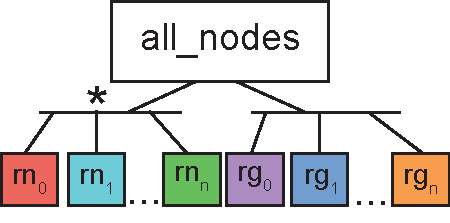
\includegraphics[scale=0.50]{figs/OwnedTree.pdf}
}
\subfigure[Circuit piece coloring.]{
\label{sfig:part_fig:pieces}
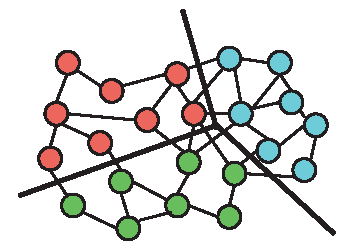
\includegraphics[scale=0.67]{figs/Owned_Nodes.pdf}
}
\subfigure[Ghost {\tt rg0} coloring.]{
\label{sfig:part_fig:ghost_zero}
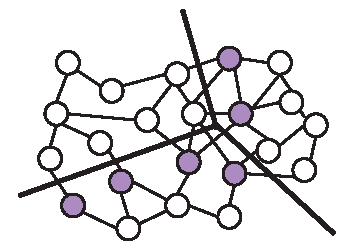
\includegraphics[scale=0.67]{figs/Ghost_RN0.pdf}
}
\subfigure[Ghost {\tt rg1} coloring.]{
\label{sfig:part_fig:ghost_one}
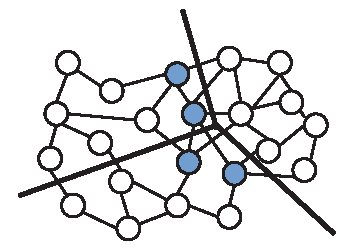
\includegraphics[scale=0.67]{figs/Ghost_RN1.pdf}
}
\vspace{-2mm} 
\caption{Partitions of $r{\_}all{\_}nodes$. \label{fig:part_fig}}
\vspace{-6mm}
%  \caption[My caption
\end{figure}

To efficiently support the access patterns of the circuit simulation,
the {\tt all\_nodes} region is partitioned in two different ways.  The
desired {\em region tree} is shown in Figure~\ref{sfig:part_fig:tree}.
First, there are {\em subregions} of {\tt all\_nodes} that describe
the set of nodes ``owned'' by each piece, called {\tt rn0}, {\tt rn1},
$\ldots$. Since each node is in one piece, this partition is {\em
disjoint} (indicated by a $*$ on the left subtree).
Figure~\ref{sfig:part_fig:pieces} shows one possible node partition;
different colors identify different piece IDs.  Second, each piece of
the circuit needs access to the nodes on its border, commonly referred
to as {\em ghost nodes}.  The ghost nodes for two circuit pieces are
shown in Figures~\ref{sfig:part_fig:ghost_zero}
and~\ref{sfig:part_fig:ghost_one}; note two nodes are in both sets.
Because a node may neighbor more than one other circuit piece, this
second partition of {\tt all\_nodes} is {\em aliased}.  Thus, there
are two sources of aliasing in the region tree: the two distinct partitions
divide the {\tt all\_nodes} region in different ways, and the ghost
node subregions are not disjoint.

Note there are two alternative approaches to using multiple partitions,
both of which avoid introducing aliasing:
first, we could create a single partition with $2^n$ subregions, one for each
possible case of sharing; second, tasks for each piece could use the
{\tt all\_nodes} region to access their ghost nodes.  Neither option
is attractive: the former significantly complicates programming, the
latter greatly increases runtime data movement and would limit parallelism.

Programmers express partitions using {\em colorings},
maps from region elements to integers (``colors'').
Listing~\ref{lst:coloring} shows the function {\tt create\_piece\_coloring}
that constructs a coloring from the piece IDs of a list of nodes.
%The coloring of wires is similar, with each wire
%using the color of its first endpoint.  
For aliased partitions such as the ghost nodes, a {\em multicoloring}
is used, which assigns each region element to one or more colors.  
%(Multicolorings are
%implemented in Core Legion with separate colorings for each color.)
\begin{lstlisting}[label={lst:coloring},caption={Coloring Construction}]
function create_piece_coloring[rl,rn](node_list: NodeList<rl,rn>@rl),
            reads(rl,rn) : coloring(rn) = 
    if isnull(node_list) then
        newcolor(rn) 
    else                                 -- tuple fields accessed by .(field number)
        let list_elem : NodeList<rl,rn> = read(node_list) in
        let part_coloring : coloring(rn) = create_node_coloring(list_elem.2) in
        let node : CircuitNode = read(list_elem.1) in
            color(part_coloring, list_elem.1, node.5)
\end{lstlisting}

Colorings are the input to partition operations in Legion.  The partition
statement shown in Listing~\ref{lst:partition} performs the ``owned nodes''
partitioning.    Since colorings assign each region element at most one color
(dynamically checked), the partition operation results in 
{\em disjoint} subregions, each a subset of the {\em parent} region.
A partition operation introduces constraints into the static type environment describing
both the disjointness of subregions (e.g., {\tt rn0 $*$ rn1})
and the subregion relationships
(e.g., {\tt rn0 $\leq$ all\_nodes}).  A partition created from a multicoloring
only introduces the subregion relationships, as the partition may be aliased.



%The partitioning of wires is identical, while the partitioning
%of the ghost nodes is performed in Core Legion as a separate partitioning operation
%for each color.

\begin{lstlisting}[label={lst:partition},caption={Partition Operation Example}]
let piece_coloring : coloring(all_nodes) = create_piece_coloring[rl,all_nodes](node_list) in
partition all_nodes using piece_coloring as rn0,rn1... in ...
\end{lstlisting}


%% In addition, to partitioning the graph to describe {\em owned} nodes
%% for each piece, the circuit example also
%% needs to be able to name the {\em ghost nodes} for each piece.  Ghost node
%% regions are used for accessing the nodes of wires that span
%% two different pieces. (This is also the reason {\tt CircuitWire} is parametrized on
%% two regions).  Figure~\ref{sfig:part_fig:ghost_zero} and 
%% Figure~\ref{sfig:part_fig:ghost_one} show colorings for the ghost regions
%% corresponding to {\tt rn0} and {\tt rn1} respectively.  Note that two 
%% nodes are colored in both colorings.  Since nodes can appear in multiple
%% subregions, we use a {\em multicoloring} (implemented in core Legion
%% by multiple single colorings) to describe {\em aliased} partitions.  Aliased
%% partitions still introduce subregion constraints into the static checking
%% environment, but not disjointness constraints.  Figure~\ref{sfig:part_fig:tree}
%% shows the resulting logical region tree for node regions.

The first-class nature of logical regions in Legion allows them to
be written into the heap.  To avoid losing information about these regions and pointers
into those regions, Legion provides {\em region
relationships}.  Region relationships are a bounded existential type
that allows programmers to {\em pack} a group of regions and pointers together and capture
properties about them such as disjointness and subregion relationships.
Listing~\ref{lst:rr} shows an example region relationship for a {\tt CircuitPiece} 
describing its region of wires {\tt rpw}, region of 
nodes {\tt rpn}, region of ghost nodes {\tt rg}, and important constraints.  Although the
``names'' of {\tt rpw}, {\tt rpn}, and {\tt rg} are lost when packed into the region relationship,
the knowledge that they are subregions of the {\tt rw} and {\tt rn} regions is not.

\begin{lstlisting}[label={lst:rr},caption={Region Relationship Example}]
type CircuitPiece<rl,rw,rn> = rr[rpw,rpn,rg]  -- rr is keyword for region relationship 
                            < WireList<rl,rpw,rpn,rg>@rl, NodeList<rl,rpn>@rl >         
                            where rpn #$\le$# rn and rg #$\le$# rn and rpw #$\le$# rw and
                                  rn * rw and rl * rn and rl * rw
\end{lstlisting}

The Legion type system verifies properties of region relationships when packing.  When
a region relationship is unpacked later, fresh names are given to the regions that were
captured by the region relationship (passed in {\tt []} parameters), and the properties that are known to hold for these
regions are re-introduced to the type environment.
In contrast, region access privileges cannot be packed in a region
relationship---privileges belong to functions. When a function unpacks
a region relationship it must already hold privileges for the unpacked regions it wishes to access.

Listing~\ref{lst:loop} shows the main time step loop run by the 
recursive function {\em execute\_time\_steps} (line 11)
as well the leaf task functions (lines 2-7).  
For each time step, the loop unpacks 
two previously packed circuit pieces, giving new names to the subregions introduced
by each region relationship.  The {\em execute\_time\_steps} function
will have read/write privileges for the newly named regions, such as {\tt rn0},
because it has read/write privileges for {\tt rn} and the {\tt CircuitPiece} 
region relationship ensures that {\tt rn0 $\leq$ rn}.

The {\tt execute\_time\_steps} function   
illustrates the importance of having different partitions provide 
multiple views onto the same logical region.  Both {\tt calc\_new\_currents} 
and {\tt distribute\_charge} (lines 2-5)
use the owned and ghost regions of a piece, which are from different partitions. In
{\tt calc\_new\_currents} these regions only need read
privileges, allowing both instances of the task to be
run in parallel.  In {\tt distribute\_charge} the
privilege is for a reduction which can also be done in parallel
because of the atomic and commutative nature of reductions.  Finally,
the {\tt update\_voltage} function (line 6) modifies only the disjoint owned regions, 
permitting each piece to be updated in parallel.  No single partition of the nodes
describes these data sharing patterns.

\lstset{
  captionpos=b,
  language=Haskell,
  basicstyle=\scriptsize,
  numbers=left,
  numberstyle=\tiny,
  columns=fullflexible,
  stepnumber=1,
  escapechar=\#,
  keepspaces=true,
  belowskip=-10pt,
  literate={<}{{$\langle$}}1 {>}{{$\rangle$}}1,
  morekeywords={function,rr,int,float,bool,isnull,partition,as,downregion,upregion,reads,writes,rdwrs,reduces,read,write,reduce,using,unpack,pack,coloring,multicoloring,color,newcolor,atomic,simultaneous},
  deletekeywords={head,min,max}
}
\begin{lstlisting}[float={t},label={lst:loop},caption={Main Simulation Loop}]
-- Leaf Task Declarations (implementations in appendix)
function calc_new_currents[rl,rw,rn,rg] ( ptr_list : WireList<rl,rw,rn,rg>@rl ), 
      reads(rl,rw,rn,rg), writes(rw) : bool
function distribute_charge[rl,rw,rn,rg] ( ptr_list : WireList<rl,rw,rn,rg>@rl ), 
      reads(rl,rw,rn), reduces(reduce_charge,rn,rg), atomic(rn,rg) : bool 
function update_voltage[rl,rn] ( ptr_list : NodeList<rl,rn>@rl ), 
      reads(rl,rn), writes(rn) : bool
-- Reduction function for distribute charge
function reduce_charge ( node : CircuitNode, current : float ) : CircuitNode

-- Time Step Loop
function execute_time_steps[rl,rw,rn] ( p0 : CircuitPiece<rl,rw,rn>, 
      p1 : CircuitPiece<rl,rw,rn>, steps : int ) , reads(rn,rw,rl), writes(rn,rw) : bool = 
  if steps #$<$# 1 then true else
  unpack p0 as piece0 : CircuitPiece<rl,rw,rn>[rw0,rn0,rg0] in 
  unpack p1 as piece1 : CircuitPiece<rl,rw,rn>[rw1,rn1,rg1] in
  let _ : bool = calc_new_currents[rl,rw0,rn0,rg0](piece0.1) in
  let _ : bool = calc_new_currents[rl,rw1,rn1,rg1](piece1.1) in
  let _ : bool = distribute_charge[rl,rw0,rn0,rg0](piece0.1) in
  let _ : bool = distribute_charge[rl,rw1,rn1,rg1](piece1.1) in
  let _ : bool = update_voltage[rl,rn0](piece0.2) in
  let _ : bool = update_voltage[rl,rn1](piece1.2) in
      execute_time_steps[rl,rw,rn](p0,p1,steps-1)
\end{lstlisting}

The {\tt execute\_time\_steps} function also demonstrates the need to 
dynamically discover parallelism through region disjointess.  
To run the two instances of 
{\tt calc\_new\_currents} in parallel requires knowing that {\tt rw0}
and {\tt rw1} are disjoint (lines 17-18).  There is a similar requirement for parallel
execution of the two {\tt update\_voltage} calls with {\tt rn0} and {\tt rn1} (lines 21-22).  In
both cases, this knowledge was statically available when the subregions were created 
and could have been captured in a region relationship at the cost
of much more complicated code.  Instead, we use a simpler region relationship
and rely on an inexpensive dynamic disjointness
check by the Legion runtime to (re)discover the parallelism.

In addition to privileges, functions can also specify {\em coherence}
on regions.  By default, coherence on all regions is {\em exclusive}, meaning
the function must appear to execute in program order relative to other function
calls that access non-disjoint data.  Programmers can allow other
execution orderings using relaxed coherence.  Line 5 of Listing~\ref{lst:loop} shows
an example of {\tt atomic}, a relaxed coherence mode requiring
that operations to {\tt rn} and {\tt rg} appear atomic relative
to other functions using regions which may alias.  The most relaxed coherence
mode is {\tt simult}; simultaneous coherence allows concurrent access 
to the region by all functions that are using the region
in a simultaneous mode.  The interaction between {\em tasks} (which are functions 
chosen to execute in parallel) using the same region with different coherence
modes is formalized in Section~\ref{sec:coherence}.

%The most important decision in any Legion program is the choice of
%how to partition program data into logical regions.  Logical regions
%are the granularity at which the Legion runtime will reason
%about the independence of tasks, and therefore how much parallelism
%is available.  Logical regions also define the granularity at which
%the Legion runtime will move data.  Coarser regions will lead
%to more efficient bulk copies of data throgh the memory hierarchy due
%to better locality.  There is therefore a natural tension: partitioning 
%should be fine-grained enough to express desired parallelism, but not 
%so fine-grained as to result in inefficient data movement.

%The first step in the circuit example is to partition the arbitrary graph
%of circuit elements into pieces that can be handled independently.
%In the case of this example all nodes in the graph have initially
%been allocated in the region {\tt all\_nodes} (Figure~\label{sfig:part_fig:tree}).
%The decision of how to partition the graph is the responsibility
%of the programmer and can be done by an external library (e.g. METIS
%in this case).  Once the decision of how to partition is made, the
%result must be communicated to the Legion runtime to 
%generate the corresponding logical regions.  Partitioning decisions
%are described via {\em colorings}.  Colorings are parametrized by
%the region they are partitioning and capture a mapping from pointers
%into the region to specific colors (e.g. integers).  Figure~\ref{sfig:part_fig:pvs}
%illustrates the coloring used for generating the {\tt p\_nodes\_pvs}
%partition.




%
\section{Circuit Example}
\label{sec:example}

% This is a description of how the listings should be formatted.
% It can go anywhere before the listings.
\lstset{
  captionpos=b,
  language=Haskell,
  basicstyle=\scriptsize,
  numbers=left,
  numberstyle=\tiny,
  columns=fullflexible,
  stepnumber=1,
  escapechar=\#,
  keepspaces=true,
  literate={<}{{$\langle$}}1 {>}{{$\rangle$}}1,
  morekeywords={function,rr,int,float,bool,isnull,partition,as,downregion,upregion,reads,writes,rdwrs,reduces,read,write,reduce,using,unpack,pack,coloring,multicoloring,color,newcolor,atomic,simultaneous},
  deletekeywords={float,head,min,max}
}

\begin{lstlisting}[float={t},label={lst:circuit_ex},caption={Circuilt Simulation}]
-- <voltage,current,charge,capacitance>
type CircuitNode        = <float,float,float,float>
-- < owned node, owned or ghost node, resistance, current>
type CircuitWire<rn,rg>  = <CircuitNode@rn, CircuitNode@(rn,rg),float,float>

type node_list<rl,rn>       = < CircuitNode@rn, node_list<rl,rn>@rl >
type wire_list<rl,rw,rn,rg>= < CircuitWire<rn,rg>@rw, wire_list<rl,rw,rn,rg>@rl >

type CircuitPiece<rl,rw,rn> = rr[rpw,rpn,rg]
                            < wire_list<rl,rpw,rpn,rg>@rl, node_list<rl,rpn>@rl >         
                            where rpn <= rn and rg <= rn and rpw <= rw and
                                  rpn * rg and rn * rw and rl * rn and rl * rw

-- Simulation initialization and invocation
function simulate_circuit[rl,rw,rn] ( all_nodes : node_list<rl,rn>@rl, 
                            all_wires : wire_list<rl,rw,rn,rn>@rl, steps : int ), 
      reads(rn,rw,rl), writes(rn,rw,rl) : bool = 
  let pc : <coloring(rn),multicoloring(rn),coloring(rw)> 
            = color_circuit[rn,rw,rl](all_nodes,all_wires) in
  -- Disjoint partition for the owned nodes of each piece
  partition rn using pc.1 as rn0,rn1 in
  -- Aliased partition for ghost nodes of each piece
  partition rn using pc.2 as rg0,rg1 in
  -- Disjoint partition for the owned wires of each piece
  partition rw using pc.3 as rw0,rw1 in
  let lists0 : <wire_list<rl,rw0,rn0,rg0>@rl,node_list<rl,rn0>@rl> = 
        build_lists[rl,rw,rn,rw0,rn0,rg0](all_nodes,all_wires,pc.1,pc.2,pc.3,0) in
  let piece0 : CircuitPiece<rl,rw,rn> = 
        pack lists0 as CircuitPiece<rl,rw,rn>[rw0,rn0,rg0] in
  let lists1 : <wire_list<rl,rw1,rn1,rg1>@rl,node_list<rl,rn1>@rl> =
        build_lists[rl,rw,rn,rw1,rn1,rg1](all_nodes,all_wires,pc.1,pc.2,pc.3,1) in
  let piece1 : CircuitPiece<rl,rw,rn> = 
        pack lists1 as CircuitPiece<rl,rw,rn>[rw1,rn1,rg1] in
      execute_time_steps[rl,rw,rn](piece0,piece1,steps)

-- Time Step Loop
function execute_time_steps[rl,rw,rn] ( p0 : CircuitPiece<rl,rw,rn>, 
      p1 : CircuitPiece<rl,rw,rn>, steps : int ) , reads(rn,rw,rl), writes(rn,rw) : bool = 
  if steps #$<$# 1 then true else
  unpack p0 as piece0 : CircuitPiece<rl,rw,rn>[rw0,rn0,rg0] in 
  unpack p1 as piece1 : CircuitPiece<rl,rw,rn>[rw1,rn1,rg1] in
  let _ : bool = calc_new_currents[rl,rw0,rn0,rg0](piece0.1) in
  let _ : bool = calc_new_currents[rl,rw1,rn1,rg1](piece1.1) in
  let _ : bool = distribute_charge[rl,rw0,rn0,rg0](piece0.1) in
  let _ : bool = distribute_charge[rl,rw1,rn1,rg1](piece1.1) in
  let _ : bool = update_voltage[rl,rn0](piece0.2) in
  let _ : bool = update_voltage[rl,rn1](piece1.2) in
      execute_time_steps[rl,rw,rn](p0,p1,steps-1)

function color_circuit[rn,rw,rl] ( all_nodes : node_list<rl,rn>@rl, 
                               all_wires : wire_list<rl,rw,rn>@rl ), 
        reads(rn,rw,rl) : <coloring(rn), multicoloring(rn), coloring(rw)> =  
  -- Invoke programmer chosen coloring algorithm (e.g. METIS)
  -- return owned, ghost, wire colorings

-- Helper method
function build_lists[rl,rw,rn,rpw,rpn,rg] ( nodes : node_list<rl,rn>@rl, 
       wires : wire_list<rl,rw,rn>@rl, oc : coloring(rn), gc : multicoloring(rn), 
       wc : coloring(rw), c : int), reads(rn,rw,rl), writes(rl) 
       : < wire_list<rl,rpw,rpn,rg>@rl, node_list<rl,rpn>@rl > = 
  -- Construct lists of node and wire pointers for the given colorings
\end{lstlisting}

\begin{lstlisting}[float={t},label={lst:circuit_leaf},caption={Circuilt Leaf Tasks}]
function calc_new_currents[rl,rw,rn,rg] ( ptr_list : wire_list<rl,rw,rn,rg>@rl ), 
      reads(rl,rw,rn,rg), writes(rw) : bool =
  if isnull(ptr_list) then true else
  let wire_node : wire_list<rl,rw,rn,rg> = read(ptr_list) in
  let wire : CircuitWire<rn,rg> = read(wire_node.1) in
  let in_node : CircuitNode = read(wire.1) in
  let out_node : CircuitNode = read(wire.2) in
  let current : float = (in_node.1 - out_node.1) /  wire.3 in 
  let new_wire : CircuitWire<rn,rg> = <wire.1,wire.2,wire.3,current> in
  let _ : CircuitWire<rn,rg>@rw = write(wire_node.1, new_wire) in
      calc_new_currents[rl,rw,rn,rg](wire_node.2)

function distribute_charge[rl,rw,rn,rg] ( ptr_list : wire_list<rl,rw,rn,rg>@rl ), 
      reads(rl,rw,rn), reduces(reduce_charge,rn,rg), atomic(rn,rg) : bool =
  if isnull(ptr_list) then true else
  let wire_node : wire_list<rl,rw,rn,rg> = read(ptr_list) in
  let wire : CircuitWire<rn,rg> = read(wire_node.1) in
  let _ : CircuitNode@rn = reduce(reduce_charge, wire.1, wire.4) in
  let _ : CircuitNode@(rn,rg) = reduce(reduce_charge, wire.2, wire.4) in
      distribute_charge[rl,rw,rn,rg](wire_node.2)

function update_voltage[rl,rn] ( ptr_list : node_list<rl,rn>@rl ), 
      reads(rl,rn), writes(rn) : bool = 
  if isnull(ptr_list) then true else
  let node_node : node_list<rl,rn> = read(ptr_list) in
  let node : CircuitNode = read(node_node.1) in
  let voltage : float = (node.3/node.4) in
  let new_node : CircuitNode = <voltage,node.2,node.3,node.4> in
  let _ : CircuitNode@rn = write(node_node.1, new_node) in
      update_voltage[rl,rn](node_node.2)

-- Reduction function for distribute charge
function reduce_charge ( node : CircuitNode, current : float ) : CircuitNode =
    let new_charge : float = node.3 + current in
        < node.1,new_charge,node.3,node.4>
\end{lstlisting}



%\section{Outline}

\begin{enumerate}
\item Abstract
\item Introduction
\item LLR Components
  \begin{enumerate}
  \item Processors
  \item Memories
  \item Events
  \item Locks
  \item Physical Regions
  \end{enumerate}
\item Implementations
  \begin{enumerate}
  \item SMP Version
  \item GASNet/CUDA Version
  \end{enumerate}
\item Microbenchmarks
  \begin{enumerate}
  \item Events
    \begin{enumerate}
    \item Latency (inter- and intra-node)
    \item Throughput (separate tracks and single wide track)
    \end{enumerate}
  \item Locks
    \begin{enumerate}
    \item Latency, Throughput vs. Load
    \item Locality - associate data with lock either implicitly or explicitly, show effect of unfairness
    \end{enumerate}
  \item Reductions
    \begin{enumerate}
    \item Histogram Mini-app - vary data, histogram sizes, use variety of reduction techniques
    \end{enumerate}
  \end{enumerate}
\item Applications
  \begin{enumerate}
  \item Circuit
  \item Fluid
  \item AMR
  \end{enumerate}
\item Application Profiling
  \begin{enumerate}
  \item Events
    \begin{enumerate}
    \item Lifetimes (Storage Cost)
    \item Trigger vs. Query Times
    \item Waiters per Event (individual and aggeregated per-node)
    \end{enumerate}
  \item Locks
    \begin{enumerate}
    \item ???
    \end{enumerate}
  \item Reductions
    \begin{enumerate}
    \item ???
    \end{enumerate}
  \item Deferred Execution
    \begin{enumerate}
    \item Comparison vs. Bulk Synchronous Implementation
    \end{enumerate}
  \end{enumerate}
\item Related Work
\item Conclusion
\item Bibliography
\end{enumerate}

\section{TODO}

\newcommand{\tblhdr}[1]{\multicolumn{1}{c}{\bf #1}}

\begin{tabular}{lll}
\tblhdr{Status} & \tblhdr{Owner} & \tblhdr{Task} \\
DONE & Mike & Code event latency microbenchmark \\
& Mike & Code event throughput microbenchmark \\
& ?? & Code lock latency/throughput microbenchmark \\
& Sean & Code lock locality microbenchmark \\
& ?? & Code histogram microbenchmark \\
& Sean & Detailed event logging \\
& Sean & Bulk-Synchronous Mode: Circuit \\
& Sean & Bulk-Synchronous Mode: Fluid \\
& Mike & Bulk-Synchronous Mode: AMR \\
\end{tabular}


\newtheorem{thm}{Theorem}
\newtheorem{lem}{Lemma}

\newcommand{\oton}[1]{{#1}_1,\ldots,{#1}_n}
\newcommand{\otok}[2]{{#2}_1,\ldots,{#2}_{#1}}
\newcommand{\dplus}{\text{+\!+}}
\newcommand{\llbracket}{[\![}
\newcommand{\rrbracket}{]\!]}
\newcommand{\tuple}[2]{\langle #1, #2 \rangle}
\makeatletter
% macros for consistency flavors
\newcommand{\simH}{\sim_{\!H}}
% usually: \mapconsist{\Omega}
\newcommand{\mapconsist}[2][M]{#1 \sim #2}
% usually: \localconsist{L}{\Gamma}
\newcommand{\localconsist}[3][M]{#2 \simH \@ifmtarg{#1}{#3}{#1 \llbracket #3 \rrbracket}}
% usually: \storeconsist{S}{H}
\newcommand{\storeconsist}[2]{#1 \sim #2}
% usually: \valueconsist{v}{T}
\newcommand{\valueconsist}[3][M]{#2 \simH \@ifmtarg{#1}{#3}{#1 \llbracket #3 \rrbracket}}
% usually: \traceconsist{E}
\newcommand{\traceconsist}[2][H]{#2 \sim #1}
% usually: \privconsist{E}{\Phi}
\newcommand{\privconsist}[3][M]{#2 \@ifmtarg{#1}{:}{:_{\!#1}} #3}

\newcommand{\nonint}[1][]{\#\@ifmtarg{#1}{}{_{\!\!#1}}}
\makeatother

% override BCP's typesetrule function to left-justify multiple lines of hypotheses
\renewcommand{\typesetrule}[2]{%
   \setrulebody{%
      \frac{\begin{array}{@{}l@{}}#1\end{array}}%
           {\begin{array}{@{}l@{}}#2\end{array}}}}

% fun latex tricks to make typeenv and opsenv more friendly
\makeatletter
\define@key{typeenv}{G}{\def\typeenv@G{#1}}
\define@key{typeenv}{P}{\def\typeenv@P{#1}}
\define@key{typeenv}{O}{\def\typeenv@O{#1}}
\newcommand{\typeenvx}[1][]{
{
% default values
\def\typeenv@G{\Gamma}
\def\typeenv@P{\Phi}
\def\typeenv@O{\Omega}
\setkeys{typeenv}{#1}
\typeenv@G, \typeenv@P, \typeenv@O \vdash \,
}}
\newcommand{\typeenv}[3][]{\typeenvx[#1] {#2} : {#3}}
\define@key{opsenv}{M}{\def\opsenv@M{#1}}
\define@key{opsenv}{L}{\def\opsenv@L{#1}}
\define@key{opsenv}{H}{\def\opsenv@H{#1}}
\define@key{opsenv}{S}{\def\opsenv@S{#1}}
\define@key{opsenv}{C}{\def\opsenv@C{#1}}
\newcommand{\opsenvx}[1][]{
{
% default values
\def\opsenv@M{M}
\def\opsenv@L{L}
\def\opsenv@H{H}
\def\opsenv@S{S}
\def\opsenv@C{C}
\setkeys{opsenv}{#1}
\opsenv@M, \opsenv@L, \opsenv@H, \opsenv@S, \opsenv@C \vdash \,
}}
\newcommand{\opsenv}[4][]{\opsenvx[#1] {#2} \mapsto {#3}, {#4}}
\makeatother

\begin{figure*}
\centering
{\small
\begin{tabular}{cclr|cclr}

$T$ & ::= &  & types & $bv$ & ::= & false $\;\;\;\mid\;\;\;$ true & \\
  &$\mid$& bool $\;\;\;\mid\;\;\;$ int & base types & & & & \\
  &$\mid$& $\langle T_1, T_2 \rangle$ & tuple & $iv$ & ::= & 0 $\;\;\;\mid\;\;\;$ 1 $\ldots$ & \\
  &$\mid$& $T@(\oton{r})$ & pointer & & & & \\
  &$\mid$& $\text{coloring}(r)$ & region coloring & $e$ & ::= & & expressions \\
  &$\mid$& $\exists \oton{r}. T\text{ where }\Omega$ & region relationship &   &$\mid$& $bv$ $\;\;\;\mid\;\;\;$ $iv$ & constants \\
  &$\mid$& $\forall \oton{r}. (\oton{T}), \Phi, Q \rightarrow T_r$ & functions &   &$\mid$& $\langle e_1, e_2 \rangle$ $\;\;\;\mid\;\;\;$ $e$.1 $\;\;\;\mid\;\;\;$ $e$.2 & tuple \\
& & & &   &$\mid$& $id$ &  \\
$\Omega$ & ::= & $\{ \oton{\omega} \}$ & region constraints &   &$\mid$& $\text{new}\ T@r$ $\;\;\;\mid\;\;\;$ $\text{null }T@r$ $\;\;\;\mid\;\;\;$ $\text{isnull}(e)$ & \\
$\omega$ & ::= & $r_1 \leq r_2$ & subregion   &   
  &$\mid$& $\text{upregion}(e, r_1,\ldots,r_n)$ & \\
  &$\mid$& $r_1 * r_2$ & disjointness &   
  &$\mid$ & $\text{downregion}(e, r_1,\ldots,r_n)$ & \\  
& & &  & 
  &$\mid$& $\text{read}(e_1)$ $\;\mid\;$ $\text{write}(e_1, e_2)$ & memory access \\
$\Phi$ & ::= & $\{ \oton{\phi} \}$ & privileges & 
  & $\mid$ & $\text{reduce}(id, e_1, e_2)$ & \\
$\phi$ & ::= & reads$(r)$ $\;\mid\;$ writes$(r)$ $\;\mid\;$ $\text{reduces}_{id}(r)$ &  &  
  &$\mid$& $\text{newcolor}\ r$ $\;\mid\;$ $\text{color}(e_1, e_2, e_3)$ & coloring \\
& & & &  
  &   $\mid$& $e_1 + e_2$ & integer ops \\
$Q$ & ::= & $\{ \oton{q} \}$ & coherence modes  &   
       & $\mid$& $e_1 < e_2$ & comparisons \\
$q$ & ::= & atomic$(r)$ $\;\;\;\mid\;\;\;$ simult$(r)$ & &   
  &$\mid$& $\text{let}\ id : T = e_1 \text{in}\ e_2$ &  \\
& & & &   
       & $\mid$& $\text{if}\ e_1\ \text{then}\ e_2\ \text{else}\ e_3$ &  \\
$v$ & ::= & & values &   
       & $\mid$& $id[r_1, \ldots, r_n](e_1,\ldots,e_n)$ & function calls \\
  &$\mid$& $bv$ $\;\;\;\mid\;\;\;$ $iv$ & base values &   
       & $\mid$ & $\text{partition}\ r_p\text{ using }e_1\text{ as }\oton{r}\text{ in }\ e_2$ &  \\
  &$\mid$& $\langle v_1, v_2 \rangle$ & tuple & 
       & $\mid$& $\text{pack}\ e_1\ \text{as}\ T[r_1,\ldots,r_n]$ &  \\
  &$\mid$& null $\;\;\;\mid\;\;\;$ $a$ & address & 
       & $\mid$& $\text{unpack}\ e_1\ \text{as}\ id : T[r_1,\ldots,r_n]\ \text{in}\ e_2$ &  \\
  &$\mid$& $\{ (a_i, iv), \ldots \}$ & coloring & 
    & & & \\
  &$\mid$& $\langle \langle \oton{\rho}, v\rangle \rangle$ & reg. relation instance & 
   & & & \\
%$bv$ & ::= & false $\;\;\;\mid\;\;\;$ true \\
%\\
%$iv$ & ::= & 0 $\;\;\;\mid\;\;\;$ 1 $\ldots$ \\
%\\
%$e$ & ::= & & expressions \\
%  &$\mid$& $bv$ $\;\;\;\mid\;\;\;$ $iv$ & constants \\
%  &$\mid$& $\langle e_1, e_2 \rangle$ $\;\;\;\mid\;\;\;$ $e$.1 $\;\;\;\mid\;\;\;$ $e$.2 & tuple \\
%  &$\mid$& $id$ &  \\
%  &$\mid$& $\text{new}\ T@r$ $\;\;\;\mid\;\;\;$ $\text{null }T@r$ $\;\;\;\mid\;\;\;$ $\text{isnull}(e)$ & \\
%  &$\mid$& $\text{upregion}(e, r_1,\ldots,r_n)$ $\;\;\;\mid\;\;\;$ $\text{downregion}(e, r_1,\ldots,r_n)$ & \\
%  &$\mid$& $\text{read}(e_1)$ $\;\;\;\mid\;\;\;$ $\text{write}(e_1, e_2)$ $\;\;\;\mid\;\;\;$ $\text{reduce}(id, e_1, e_2)$ & memory access \\
%  &$\mid$& $\text{newcolor}\ r$ $\;\;\;\mid\;\;\;$ $\text{color}(e_1, e_2, e_3)$ & coloring operations \\
%  &$\mid$& $e_1 + e_2$ & integer operations \\
%  &$\mid$& $e_1 < e_2$ & comparison operations \\
%  &$\mid$& $\text{let}\ id : T = e_1 \text{in}\ e_2$ &  \\
%  &$\mid$& $\text{if}\ e_1\ \text{then}\ e_2\ \text{else}\ e_3$ &  \\
%  &$\mid$& $id[r_1, \ldots, r_n](e_1,\ldots,e_n)$ & function calls \\
%  &$\mid$& $\text{partition}\ r_p\text{ using }e_1\text{ as }\oton{r}\text{ in }\ e_2$ &  \\
%  &$\mid$& $\text{pack}\ e_1\ \text{as}\ T[r_1,\ldots,r_n]$ &  \\
%  &$\mid$& $\text{unpack}\ e_1\ \text{as}\ id : T[r_1,\ldots,r_n]\ \text{in}\ e_2$ &  \\
\end{tabular}
}
\caption{Core Legion}
\label{fig:langdef}
\vspace{-5mm}
\end{figure*}

\newcommand{\placeat}[3]{%
\makebox[0pt]{%
\hspace*{#1in} \raisebox{#2in}{#3}%
}%
}

\newcommand{\infrulez}[2]{\displaystyle\frac{\displaystyle\strut{#1}}{\displaystyle\strut {#2}}}
\newcommand{\cinfrulez}[3]{\parbox{14cm}{\hfil$\infrulez{#1}{#2}$\hfil}\parbox{4cm}{$\,#3$\hfil}}
\newcommand{\finfrulez}[2]{\framebox{$\infrulez{#1}{#2}$}}

\newcommand{\ruleat}[5]{
\node[below right] at (#1) {$\infrulez{#4}{#5}$};
\node[below] at (#2) {[#3]};
}

\newcommand{\ruleatx}[5]{
\node[below right,fill=white!50] at (#1) {$\infrulez{\begin{array}{l}#4\end{array}}{#5}$};
\node[below] at (#2) {[#3]};
}

\newcommand{\axiomat}[4]{
\node[below right] at (#1) {$#4$};
\node[below] at (#2) {[#3]};
}

\begin{figure*}
{
\begin{tikzpicture}[x=1in,y={(0,-1in)}]
%\draw[thin] (0,0) to (7,0);
%\draw[thin] (0,0) to (0,6);
\foreach \y in {0,...,80}{
%  \draw[thin] (0,0.1*\y) to (7,0.1*\y);
}
\foreach \y in {0,...,16}{
%  \draw[red,thick] (0,0.5*\y) to (7,0.5*\y);
}
\foreach \y in {0,...,8}{
%  \draw[blue,very thick] (0,\y) to (7,\y);
}

\draw[very thin] (3.0,0.1) -- (3.0,7.6);
 
% start with read/write/reduce rules
\ruleat{0.0,0.0}{2.6,0.2}{T-Read}
{\begin{array}{l}
\typeenvx e_1 : T@(\oton{r}) \\
\forall i, reads(r_i) \in \Phi^*\end{array}}
{\typeenvx \text{read}(e_1) : T}

\ruleat{0.0,0.6}{2.6,0.8}{T-Write}
{\begin{array}{l}
\typeenvx e_1 : T@(\oton{r}) \\
\typeenvx e_2 : T \\
\forall i, writes(r_i) \in \Phi^*
\end{array}}
{\typeenvx \text{write}(e_1, e_2) : T@(\oton{r})}

\ruleat{0.0,1.3}{2.6,1.5}{T-Reduce}
{\begin{array}{l}
\Gamma(id) = (T_1, T_2), \emptyset, \emptyset \rightarrow T_1 \\
\typeenvx e_1 : T_1@(\oton{r}) \\
\typeenvx e_2 : T_2 \\
\forall i, reduces_{id}(r_i) \in \Phi^*
\end{array}}
{\typeenvx \text{reduce}(id, e_1, e_2) : T_1@(\oton{r})}

\axiomat{0.0,2.2}{2.6,2.2}{T-New}
{\typeenvx \text{new }T@r : T@r}

\ruleat{0.0,2.5}{2.6,2.55}{T-UpRgn}
{\begin{array}{l}
\typeenvx e : T@(r'_1, \ldots r'_k) \\
\forall i. \exists j, r'_i \leq r_j \in \Omega^* \\
\end{array}}
{\typeenvx upregion(e,\oton{r}) : T@(\oton{r})}

\ruleat{0.0,3.1}{2.6,3.05}{T-DnRgn}
{\begin{array}{l}
\typeenvx e : T@(r'_1, \ldots r'_k) \\
%\forall j. \exists i, r_j \leq r'_i \in \Omega^* \\
\end{array}}
{\typeenvx downregion(e,\oton{r}) : T@(\oton{r})}

\axiomat{0.0,3.6}{2.6,3.6}{T-NewColor}
{\typeenvx \text{newcolor }r : \text{coloring}(r)}

\ruleat{0.0,3.9}{2.6,4.1}{T-Color}
{\begin{array}{l}
\typeenvx e_1 : \text{coloring}(r) \\
\typeenvx e_2 : T@r \\
\typeenvx e_3 : int
\end{array}}
{\typeenvx \text{color}(e_1, e_2, e_3) : \text{coloring}(r)}

\ruleat{0.0,4.6}{2.6,4.55}{T-Partition}
{\begin{array}{l}
\typeenvx e_1 : \text{coloring}(r_p) \\
\Omega' = \Omega \wedge \bigwedge_{i \in [1,k]} r_i \leq r_p \wedge \bigwedge_{1 \leq i < j \leq k} r_i * r_j \\
\typeenvx[O=\Omega'] e_2 : T \\
\{ \oton{r} \} \cap \textit{regions\_of}(\Gamma, T) = \emptyset
\end{array}}
{\typeenvx \text{partition}\ r_p\text{ using }e_1\text{ as }\otok{k}{r}\text{ in }e_2 : T}

\ruleat{0,5.5}{2.6,5.7}{T-Pack}
{\begin{array}{l}
T_1 = \exists r'_1, \ldots r'_n.\ T_2\text{ where }\Omega_1 \\
\Omega_1[r_1/r'_1,\ldots,r_k/r'_k] \subseteq \Omega^* \\
\typeenvx e_1 : T_2[r_1/r'_1,\ldots,r_k/r'_k]
\end{array}}
{\typeenvx \text{pack}\ e_1\ \text{as}\ T_1[\otok{k}{r}] : T_1}

\ruleat{0.0,6.2}{2.6,6.4}{T-Unpack}
{\begin{array}{l}
T_1 = \exists r'_1, \ldots, r'_n.\ T_2\text{ where }\Omega_1 \\
\typeenvx e_1 : T_1 \\
\Gamma' = \Gamma[T_2[r_1/r'_1,\ldots,r_k/r'_k] / id] \\
\Omega' = \Omega \cup \Omega_1[r_1/r'_1,\ldots,r_k/r'_k] \\
\typeenvx[G=\Gamma',O=\Omega'] e_2 : T_3 \\
\{ \oton{r} \} \cap \textit{regions\_of}(\Gamma, T_1, T_3) = \emptyset
\end{array}}
{\typeenvx \text{unpack}\ e_1\ \text{as}\ id : T_1[\otok{k}{r}] \text{in}\ e_2 : T_3}

\ruleat{0.0,7.4}{2.6,7.6}{T-Call}
{\begin{array}{l}
\Gamma(id) = \forall r'_1, \ldots r'_k.(\oton{T}),\Phi', Q' \rightarrow T_r \\
\typeenvx e_i : T_i[r_1/r'_1,\ldots,r_k/r'_k] \\
\Phi'[r_1/r'_1,\ldots,r_k/r'_k] \subseteq \Phi^*
\end{array}}
{\typeenvx id[\otok{k}{r}](\oton{e}) : T_r[r_1/r'_1,\ldots,r_k/r'_k]}

% now the operational semantics versions

\ruleatx{3.1,0.0}{6.7,0.2}{E-Read}{
\opsenvx e \mapsto l, E \andalso S' = \text{apply}(S, E) \\
v = \begin{cases} S'(l), & \text{if } l \not\in C \\
v' : H(l), & \text{otherwise} \end{cases}
}{\opsenvx \text{read}(e) \mapsto v, E \dplus [ read(l, excl, v) ]}

\ruleatx{3.1,0.9}{6.7,0.85}{E-Write}{
\opsenvx e_1 \mapsto l, E_1 \andalso S' = \text{apply}(S, E_1) \\
\opsenvx[S=S'] e_2 \mapsto v, E_2 \andalso valid\_interleave(S, C, E', E_1, E_2)
}{\opsenvx \text{write}(e_1, e_2) \mapsto l, E' \dplus [ write(l, excl, v) ]}

\ruleatx{3.1,1.5}{6.7,1.45}{E-Reduce}{
\opsenvx e_1 \mapsto l, E_1 \andalso S' = \text{apply}(S, E_1) \\
\opsenvx[S=S'] e_2 \mapsto v, E_2 \andalso valid\_interleave(S, C, E', E_1, E_2)
}{\opsenvx \text{reduce}(id, e_1, e_2) \mapsto l, E' \dplus [ reduce_{id}(l, excl, v) ]}

\ruleatx{3.1,2.1}{6.7,2.2}{E-New}{
l \in M(r) \andalso
H(l) = M \llbracket T \rrbracket
}{\opsenvx \text{new }T@r \mapsto l, []}

\ruleat{3.1,2.6}{6.7,2.7}{E-UpRgn}{
\opsenvx e \mapsto v, E
}{\opsenvx \text{upregion}(e, \oton{r}) \mapsto v, E}

\ruleatx{3.1,3.1}{6.7,3.3}{E-DnRgn}{
\opsenvx e \mapsto l, E \\
v = \begin{cases} l, & \text{if $\exists i, l \in M(r_i)$}. \\ null, & \text{otherwise}. \end{cases}
}{\opsenvx \text{downregion}(e, \oton{r}) \mapsto v, E}

\ruleatx{3.1,4.0}{6.7,4.2}{E-NewColor}{
K = \{ (l_1, iv_1), \ldots, (l_p, iv_p) \}, \text{ where } \\
(\forall i \in [1,p]. l_i \in M(r)) \wedge (\forall i,j \in [1,p]. l_i \not= l_j)
}{\opsenvx \text{newcolor }r \mapsto K, []}

\ruleatx{3.1,4.7}{6.7,4.9}{E-Color}{
\opsenvx e_1 \mapsto K, E_1 \andalso S' = \text{apply}(S, E_1) \\
\opsenvx[S=S'] e_2 \mapsto l, E_2 \andalso S'' = \text{apply}(S', E_2) \\
\opsenvx[S=S''] e_3 \mapsto v, E_3 \\
K' = \{ (l,v) \} \cup \{ (l_i,v_i) : (l_i,v_i) \in K \wedge l \not= l_i \} \\
valid\_interleave(S, C, E', E_1, E_2, E_3)
}{\opsenvx \text{color}(e_1, e_2, e_3) \mapsto K', E'} 

\ruleatx{3.1,5.7}{6.7,5.55}{E-Partition}{
\opsenv{e_1}{K}{E_1} \andalso \rho_i = \{ l : (l, i) \in K \}, \text{ for } 1 \leq i \leq k \\
M' = M[\rho_1/r_1, \ldots, \rho_k/r_k] \andalso S' = \text{apply}(S, E_1) \\
\opsenvx[M=M',S=S'] e_2 \mapsto v, E_2 \andalso valid\_interleave(S, C, E', E_1, E_2)
}{\opsenvx \text{partition}\ r_p\text{ using }e_1\text{ as }\otok{k}{r}\text{ in }e_2 \mapsto v, E'}

\ruleatx{3.1,6.5}{6.7,6.6}{E-Pack}{
\opsenvx e_1 \mapsto v, E \andalso \rho_i = M[r_i], \text{ for } 1 \leq i \leq k \\
v' = \langle \langle \otok{k}{\rho}, v \rangle \rangle
}{\opsenvx \text{pack}\ e_1\ \text{as}\ T_1[\otok{k}{r}] \mapsto v', E}

\ruleatx{3.1,7.1}{6.7,6.95}{E-Unpack}{
\opsenvx e_1 \mapsto \langle \langle \otok{k}{\rho} , v_1 \rangle \rangle, E_1 \andalso M' = M[\rho_1/r_1, \ldots, \rho_k/r_k] \\
L' = L[v_1/id] \andalso S' = \text{apply}(S, E_1) \\
\opsenvx[M=M',L=L',S=S'] e_2 \mapsto v_2, E_2 \andalso valid\_interleave(S, C, E', E_1, E_2)
}{\opsenvx \text{unpack}\ e_1\ \text{as}\ id : T_1[\otok{k}{r}] \text{in}\ e_2 \mapsto v_2, E'}

\ruleatx{0.0,8.1}{6.7,8.4}{E-Call}{
\opsenvx e_1 \mapsto v_1, E_1 \andalso S_1 = \text{apply}(S, E_1) \andalso \opsenvx e_2 \mapsto v_2, E_2 \andalso \ldots \andalso S_n = \text{apply}(S_{n-1}, E_n) \\
valid\_interleave(S, C, E', \oton{E}) \andalso \text{function }id[\otok{k}{r'}](a_1 : T_1, \ldots, a_n : T_n), \Phi', Q' : T_r = e_{n+1} \\
M' = \{ (r'_1, M(r_1)), \ldots (r'_k, M(r_k)) \} \andalso L' = \{ (a_1, v_1), \ldots, (a_n, v_n) \} \andalso S' = \text{apply}(S, E') \\
C' = C \cup \{ l : \exists \rho. atomic(\rho) \in M' \llbracket Q' \rrbracket \vee simult(\rho) \in M' \llbracket Q' \rrbracket \} \\
\opsenvx[M=M',L=L',S=S',C=C'] e_{n+1} \mapsto v_{n+1}, E_{n+1} \andalso E'_{n+1} = mark\_coherence(E_{n+1}, M' \llbracket Q' \rrbracket) \andalso valid\_interleave(S, C, E'', E', E_{n+1})
}{\opsenvx id[\otok{k}{r}](\oton{e}) \mapsto v_{n+1}, E''}

\end{tikzpicture}
\vspace*{-0.5cm}
\texcomment{
\framebox[7in]{
\placeat{2}{3}{bar}%
\placeat{3}{1}{3,1}%
\placeat{-3}{1}{-3,1} %
\makebox[0pt]{%
\hspace*{2in} \raisebox{3in}{---}%
} %
\makebox[0pt]{%
\hspace*{1in} \raisebox{1in}{foo}%
} %
\makebox[0pt]{%
\hspace*{2in} \raisebox{3in}{bar}%
}%
\rule{0.1pt}{6in}
}}
}
\caption{Type System and Operational Semantics Rules}
\label{fig:langrules}
\end{figure*}

%\newcommand{\infrule}[2]{\displaystyle\frac{\displaystyle\strut{#1}}{\displaystyle\strut {#2}}}
%\newcommand{\cinfrule}[3]{\parbox{14cm}{\hfil$\infrule{#1}{#2}$\hfil}\parbox{4cm}{$\,#3$\hfil}}
%\newcommand{\finfrule}[2]{\framebox{$\infrule{#1}{#2}$}}
%\newcommand{\oldfinfrule}[2]{\vspace{10pt}\framebox{$\infrule{#1}{#2}$}\vspace{10pt}}

%\newcommand{\infx}[2]{\infrule{\begin{array}{l}{#1}\end{array}}{#2}}

\section{Legion}
\label{sec:legioncore}

Figure~\ref{fig:langdef} defines Core Legion, a subset of the full Legion language
that still illustrates all of the important issues.  Types
include booleans, integers, tuples, and pointers.  Pointers
are annotated with a list of regions---a non-null pointer must point to a 
location that is contained in at least one of the regions. There is a special
type for {\em colorings}, which
are used to specify partitions of regions into subregions.
Functions in Legion are named, accept one or more arguments and
return a value of some type.  A function also declares the region
access privileges and coherence it requires.  A function may be executed
within the current task or run in parallel as a separate subtask---this decision is made
by the Legion task scheduler.  Function types are
universally quantified over all region names appearing in the type.
The final type is a region relationship, an instance of which captures a value and
one or more regions satisfying associated constraints.  A region relation instance
can be written into the heap and later read and
unpacked, giving new local names to the regions contained in
the instance.

To achieve high performance in the presence of aliasing, the Legion type system has 
been designed to efficiently leverage both static and dynamic checks.
Consequently, both the type system and the operational
semantics have been extended in interesting ways from a basic expression language.  We
describe these extensions in the next two subsections, and explain how they 
were chosen to preserve a straightforward proof of soundness for the type system.

\subsection{Core Type System}
\label{subsec:coretypes}

Core Legion is explicitly typed using judgments of the form
$$\typeenv{e}{T}$$

In addition to the traditional type environment $\Gamma$, a Legion type judgment includes the
set of access privileges $\Phi$ for the logical regions in the expression as well as a set of
constraints $\Omega$ that must hold between those logical regions.

Both $\Phi$ and $\Omega$ are used in the heap access expressions: {\em read}, {\em write}, and {\em reduce}.
For a heap access to be valid, the the appropriate permission must exist for logical region(s) in the
pointer's type.  As regions are hierarchical, the exact region need not be named in $\Phi$ if permissions
exist for a logical region that is known to contain the pointer's region.  To simplify this check, we
define closure operations in Figure~\ref{fig:closure} that expand $\Omega$ into an $\Omega^*$, which is
then used to expand $\Phi$ into a $\Phi^*$ that does explicitly name every logical region for which
privileges are known to exist.

Core Legion provides no automatic pointer type conversions.  Valid pointers are created via the {\em new}
expression in specified region and invalid (i.e. {\em null}) pointers must also be typed.  Pointers can be
``upcast'' via the {\em upregion} expression, which uses the expanded constraints $\Omega^*$ to verify that
every possible region a pointer might point into is covered by at least one of the regions in the desired
pointer type.  In contrast, a ``downcast'' using the {\em downregion} expression must perform a dynamic
test to verify which region a run-time pointer value points into.  A static test similar to the one used
for {\em upregion} could be used to catch cases in which the downcast can never succeed at runtime, but we
have left it out for simplicity.

The introduction of constraints into $\Omega$ occurs through the use of the {\em partition} expression,
which makes use of a new type specific to Legion, a {\em coloring}.  A coloring is an opaque mapping from
pointers (which must point into the region being colored) to integer {\em color} values.  (For simplicity, 
Core Legion allows only an iterative construction of a coloring via a {\em newcolor} expression that generates
an empty map, and a {\em color} expression which adds a new entry to an existing map. The opacity of the
coloring allows for more efficient generation (and storage) of colorings as needed.)  The {\em partition} 
expression introduces names for subregions corresponding to each color in the coloring, guaranteeing that each
subregion is disjoint from the other subregions and all are included in the original region.

The {\em pack} and {\em unpack} expressions allow the storage of pointers in the heap.  Logical region names
are lexically scoped and if stored in the heap as-is, can only be read within the same scope.  A region relationship
is used instead to capture the (dynamic) physical regions while preserving the statically known constraints
between those regions.  Because the {\em pack} expression is able to verify these constraints hold when the 
region relationship value is created, the {\em unpack} expression is able to reintroduce these constraints on
the (fresh) logical region names given to the contents of an unwrapped region relationship value.

Finally, the task call expression handles the aliasing of logical region names between the caller and callee and
verifies the functional requirement that the privileges held by a called task are always a subset of those held
by the caller.  In addition to being necessary for the proof of soundness, this property is critical to
enable the hierarchical scheduling model used by the Legion runtime.

\begin{comment}
\begin{figure*}
\centering{
\framebox{$\typeenv{bv}{bool}$}
\framebox{$\typeenv{iv}{int}$}
\finfrule
{\begin{array}{l}
\typeenvx e_1 : T_1 \\
\typeenvx e_2 : T_2
\end{array}}
{\typeenvx \langle e_1, e_2 \rangle : \langle T_1, T_2 \rangle}
\finfrule{\typeenvx e : \langle T_1,T_2 \rangle}{\typeenvx e\text{.1}\ : T_1}
\finfrule{\typeenvx e : \langle T_1,T_2 \rangle}{\typeenvx e\text{.2}\ : T_2}
\finfrule{\Gamma(id) = T}{\typeenvx id : T}
\framebox{$\typeenvx \text{null }T@r : T@r$}
\framebox{$\typeenvx \text{new }T@r : T@r$}
\finfrule{\typeenvx e : T@(\oton{r})}{\typeenvx \text{isnull}(e) : bool}
\finfrule
{\begin{array}{l}
\typeenvx e : T@(r'_1, \ldots r'_k) \\
\forall i. \exists j, r'_i \leq r_j \in \Omega^* \\
\end{array}}
{\typeenvx upregion(e,\oton{r}) : T@(\oton{r})}
\finfrule
{\begin{array}{l}
\typeenvx e : T@(r'_1, \ldots r'_k) \\
\forall j. \exists i, r_j \leq r'_i \in \Omega^* \\
\end{array}}
{\typeenvx downregion(e,\oton{r}) : T@(\oton{r})}
\finfrule
{\begin{array}{l}
\typeenvx e_1 : T@(\oton{r}) \\
\forall i, reads(r_i) \in \Phi^*\end{array}}
{\typeenvx \text{read}(e_1) : T}
\finfrule
{\begin{array}{l}
\typeenvx e_1 : T@(\oton{r}) \\
\typeenvx e_2 : T \\
\forall i, writes(r_i) \in \Phi^*
\end{array}}
{\typeenvx \text{write}(e_1, e_2) : T@(\oton{r})}
\finfrule
{\begin{array}{l}
\Gamma(id) = (T_1, T_2), \emptyset, \emptyset \rightarrow T_1 \\
\typeenvx e_1 : T_1@(\oton{r}) \\
\typeenvx e_2 : T_2 \\
\forall i, reduces_{id}(r_i) \in \Phi^*
\end{array}}
{\typeenvx \text{reduce}(id, e_1, e_2) : T_1@(\oton{r})}
\framebox{$\typeenvx \text{newcolor }r : \text{coloring}(r)$}
\finfrule{\begin{array}{l}
\typeenvx e_1 : \text{coloring}(r) \\
\typeenvx e_2 : T@r \\
\typeenvx e_3 : int
\end{array}}
{\typeenvx \text{color}(e_1, e_2, e_3) : \text{coloring}(r)}
\finfrule{\begin{array}{l}\typeenvx e_1 : int \\ \typeenvx e_2 : int\end{array}}{\typeenvx e_1 + e_2 : int}
\finfrule{\begin{array}{l}\typeenvx e_1 : int \\ \typeenvx e_2 : int\end{array}}{\typeenvx e_1 < e_2 : bool}
\finfrule{\begin{array}{l}
\typeenvx e_1 : T_1 \\
\typeenvx[G={\Gamma[id/T_1]}] e_2 : T_2
\end{array}}
{\typeenvx : \text{let}\ id : T_1 \text{in}\ e_2 : T_2}
\finfrule{\begin{array}{l}\typeenvx e_1 : bool \\ \typeenvx e_2 : T \\ \typeenvx e_3 : T\end{array}}{\typeenvx \text{if}\ e_1\ \text{then}\ e_2\ \text{else}\ e_3 : T}
\finfrule{
\begin{array}{l}
\Gamma(id) = \forall r'_1, \ldots r'_k.(\oton{T}),\Phi', Q' \rightarrow T_r \\
\typeenvx e_i : T_i[r_1/r'_1,\ldots,r_k/r'_k] \\
\Phi'[r_1/r'_1,\ldots,r_k/r'_k] \subseteq \Phi^*
\end{array}}
{\typeenvx id[\otok{k}{r}](\oton{e}) : T_r[r_1/r'_1,\ldots,r_k/r'_k]}
\finfrule{
\begin{array}{l}
\typeenvx e_1 : \text{coloring}(r_p) \\
\Omega' = \Omega \wedge \bigwedge_{i \in [1,k]} r_i \leq r_p \wedge \bigwedge_{1 \leq i < j \leq k} r_i * r_j \\
\typeenvx[O=\Omega'] e_2 : T \\
\{ \oton{r} \} \cap \textit{regions\_of}(\Gamma, T) = \emptyset
\end{array}}
{\typeenvx \text{partition}\ r_p\text{ using }e_1\text{ as }\otok{k}{r}\text{ in }e_2 : T}
\finfrule{
\begin{array}{l}
T_1 = \exists r'_1, \ldots r'_n.\ T_2\text{ where }\Omega_1 \\
\Omega_1[r_1/r'_1,\ldots,r_k/r'_k] \subseteq \Omega^* \\
\typeenvx e_1 : T_2[r_1/r'_1,\ldots,r_k/r'_k]
\end{array}}
{\typeenvx \text{pack}\ e_1\ \text{as}\ T_1[\otok{k}{r}] : T_1}
\finfrule{
\begin{array}{l}
T_1 = \exists r'_1, \ldots, r'_n.\ T_2\text{ where }\Omega_1 \\
\typeenvx e_1 : T_1 \\
\Gamma' = \Gamma[T_2[r_1/r'_1,\ldots,r_k/r'_k] / id] \\
\Omega' = \Omega \cup \Omega_1[r_1/r'_1,\ldots,r_k/r'_k] \\
\typeenvx[G=\Gamma',O=\Omega'] e_2 : T_3 \\
\{ \oton{r} \} \cap \textit{regions\_of}(\Gamma, T_1, T_3) = \emptyset
\end{array}}
{\typeenvx \text{unpack}\ e_1\ \text{as}\ id : T_1[\otok{k}{r}] \text{in}\ e_2 : T_3}
\finfrule{
\begin{array}{l}
\text{for }1 \leq i \leq p, \\
\Gamma(id_i) = \forall r_{i1}, \ldots r_{ik_i}. (T_{i1}, \ldots, T_{in_i}), \Phi_i, Q_i \rightarrow T_{ir} \\
\Gamma_i = \Gamma[a_{i1}/T_{i1}, \ldots, a_{in_i}/T_{in_i}] \\
\typeenv[G={\Gamma_i},P={\Phi_i},O=\emptyset]{e_i}{T_{ir}}
\end{array}}
{ 
\begin{array}{l@{ }l}
\vdash \{ & \text{function }id_1[r_{11}, \ldots, r_{1k_1}]( a_{11} : T_{11}, \ldots a_{1n_1} : T_{1n_1} ), \Phi_1, Q_1 : T_{1r} : e_1, \\
          & \ldots \\
          & \text{function }id_p[r_{p1}, \ldots, r_{pk_1}]( a_{p1} : T_{p1}, \ldots a_{pn_p} : T_{pn_p} ), \Phi_p, Q_p : T_{pr} : e_p \} : \bullet
\end{array} }
}
\caption{Legion Core Type System}
\label{fig:types}
\end{figure*}
\end{comment}

\texcomment{
\begin{figure*}
\begin{adjustwidth}{-4em}{-4em}
\begin{center}
% Row 1: bool, int, tuple1, tuple2
\begin{minipage}{\linewidth}
%\centering
\begin{tabular}{m{4cm}m{3.5cm}m{5cm}m{5cm}}
\infax[T-Bool]{\typeenv{bv}{bool}} & 
\infax[T-Int]{\typeenv{iv}{int}} & 
\infrule[T-Tuple1]{\typeenvx e : \langle T_1,T_2 \rangle}{\typeenvx e\text{.1}\ : T_1} & 
\infrule[T-Tuple2]{\typeenvx e : \langle T_1,T_2 \rangle}{\typeenvx e\text{.2}\ : T_2} 
\end{tabular}
\end{minipage}
% Row 2:  var, null, isnull, maketuple
\begin{minipage}{\linewidth}
\vspace{-0.4cm}
%\centering
\begin{tabular}{m{3cm}m{3cm}m{5cm}m{6cm}}
\infrule[T-Var]{\Gamma(id) = T}{\typeenvx id : T} &
\infax[T-Null]{\typeenvx \text{null }T@r : T@r} &
\infrule[T-IsNull]{\typeenvx e : T@(\oton{r})}{\typeenvx \text{isnull}(e) : bool} &
\infrule[T-MakeTuple]{\typeenvx e_1 : T_1 \andalso \typeenvx e_2 : T_2}{\typeenvx \langle e_1, e_2 \rangle : \langle T_1, T_2 \rangle}
\end{tabular}
\end{minipage}
% Row 3: new, newcolor, coloring
\begin{minipage}{\linewidth}
\vspace{-0.6cm}
%\centering
\begin{tabular}{m{4cm}m{5cm}m{9cm}}
\infax[T-New]{\typeenvx \text{new }T@r : T@r} &
\infax[T-Newcolor]{\typeenvx \text{newcolor }r : \text{coloring}(r)} &
\infrule[T-Color]{\typeenvx e_1 : \text{coloring}(r) \andalso \typeenvx e_2 : T@r \andalso \typeenvx e_3 : int}{\typeenvx \text{color}(e_1, e_2, e_3) : \text{coloring}(r)}
\end{tabular}
\end{minipage}
% Row 4: let, add, compare
\begin{minipage}{\linewidth}
\vspace{-0.7cm}
%\centering
\begin{tabular}{m{6cm}m{5cm}m{6cm}}
\infrule[T-Let]{\typeenvx e_1 : T_1 \\ \typeenvx[G={\Gamma[id/T_1]}] e_2 : T_2}{\typeenvx : \text{let}\ id : T_1 \text{in}\ e_2 : T_2} &
\infrule[T-Add]{\typeenvx e_1 : int \\ \typeenvx e_2 : int}{\typeenvx e_1 + e_2 : int} &
\infrule[T-Compare]{\typeenvx e_1 : int \\ \typeenvx e_2 : int}{\typeenvx e_1 < e_2 : bool}
\end{tabular}
\end{minipage}
% Row 5: upregion, downregion
\begin{minipage}{\linewidth}
\vspace{-0.4cm}
\begin{tabular}{m{9cm}m{10cm}}
\infrule[T-UpRgn]{\typeenvx e : T@(r'_1, \ldots r'_k) \andalso \forall i. \exists j, r'_i \leq r_j \in \Omega^*}{\typeenvx upregion(e,\oton{r}) : T@(\oton{r})} &
\infrule[T-DownRgn]{\typeenvx e : T@(r'_1, \ldots r'_k)
% \andalso \forall j. \exists i, r_j \leq r'_i \in \Omega^*
}{\typeenvx downregion(e,\oton{r}) : T@(\oton{r})}
\end{tabular}
\end{minipage}
% Row 6: read, write, reduce
\begin{minipage}{\linewidth}
\vspace{-0.3cm}
\begin{tabular}{m{5cm}m{5cm}m{8cm}}
\infrule[T-Read]{\typeenvx e_1 : T@(\oton{r}) \\ \forall i, reads(r_i) \in \Phi^*}{\typeenvx \text{read}(e_1) : T} &
\infrule[T-Write]{\typeenvx e_1 : T@(\oton{r}) \\ \typeenvx e_2 : T \\ \forall i, writes(r_i) \in \Phi^*}{\typeenvx \text{write}(e_1, e_2) : T@(\oton{r})} &
\infrule[T-Reduce]{\Gamma(id) = (T_1, T_2), \emptyset, \emptyset \rightarrow T_1 \andalso \typeenvx e_2 : T_2 \\
 \typeenvx e_1 : T_1@(\oton{r}) \andalso \forall i, reduces_{id}(r_i) \in \Phi^*}{\typeenvx \text{reduce}(id, e_1, e_2) : T_1@(\oton{r})}
\end{tabular}
\end{minipage}
% Row 7: pack, if-else, task call
\begin{minipage}{\linewidth}
\vspace{-0.6cm}
\begin{tabular}{m{5cm}m{5cm}m{8cm}}
\infrule[T-Pack]{T_1 = \exists r'_1, \ldots r'_n.\ T_2\text{ where }\Omega_1 \\ \Omega_1[r_1/r'_1,\ldots,r_k/r'_k] \subseteq \Omega^* \\ \typeenvx e_1 : T_2[r_1/r'_1,\ldots,r_k/r'_k]}{\typeenvx \text{pack}\ e_1\ \text{as}\ T_1[\otok{k}{r}] : T_1} &
\infrule[T-IfElse]{\typeenvx e_1 : bool \\ \typeenvx e_2 : T \\ \typeenvx e_3 : T}{\typeenvx \text{if}\ e_1\ \text{then}\ e_2\ \text{else}\ e_3 : T} &
\infrule[T-Call]{\Gamma(id) = \forall r'_1, \ldots r'_k.(\oton{T}),\Phi', Q' \rightarrow T_r \\ \typeenvx e_i : T_i[r_1/r'_1,\ldots,r_k/r'_k] \\ \Phi'[r_1/r'_1,\ldots,r_k/r'_k] \subseteq \Phi^*}{\typeenvx id[\otok{k}{r}](\oton{e}) : T_r[r_1/r'_1,\ldots,r_k/r'_k]}
\end{tabular}
\end{minipage}
% Row 8: unpack, partition
\begin{minipage}{\linewidth}
\vspace{-0.7cm}
\begin{tabular}{m{10cm}m{8cm}}
\infrule[T-Unpack]{T_1 = \exists r'_1, \ldots, r'_n.\ T_2\text{ where }\Omega_1 \andalso \typeenvx e_1 : T_1 \\
  \Gamma' = \Gamma[T_2[r_1/r'_1,\ldots,r_k/r'_k] / id] \andalso \Omega' = \Omega \cup \Omega_1[r_1/r'_1,\ldots,r_k/r'_k] \\
  \typeenvx[G=\Gamma',O=\Omega'] e_2 : T_3 \andalso \{ \oton{r} \} \cap \textit{regions\_of}(\Gamma, T_1, T_3) = \emptyset}
  {\typeenvx \text{unpack}\ e_1\ \text{as}\ id : T_1[\otok{k}{r}] \text{in}\ e_2 : T_3} &
\infrule[T-Part]{\typeenvx e_1 : \text{coloring}(r_p) \\ \Omega' = \Omega \wedge \bigwedge_{i \in [1,k]} r_i \leq r_p \wedge \bigwedge_{1 \leq i < j \leq k} r_i * r_j \\ \typeenvx[O=\Omega'] e_2 : T \\ \{ \oton{r} \} \cap \textit{regions\_of}(\Gamma, T) = \emptyset}
  {\typeenvx \text{partition}\ r_p\text{ using }e_1\text{ as }\otok{k}{r}\text{ in }e_2 : T}
\end{tabular}
\end{minipage}
% Row 9: program
\begin{minipage}{\linewidth}
\vspace{-0.5cm}
\infrule[T-Program]{\text{for }1 \leq i \leq p, \\
  \Gamma(id_i) = \forall r_{i1}, \ldots r_{ik_i}. (T_{i1}, \ldots, T_{in_i}), \Phi_i, Q_i \rightarrow T_{ir} \andalso
  \Gamma_i = \Gamma[a_{i1}/T_{i1}, \ldots, a_{in_i}/T_{in_i}] \andalso
  \typeenv[G={\Gamma_i},P={\Phi_i},O=\emptyset]{e_i}{T_{ir}}}
  {\begin{array}{@{}l@{}l@{}}
   \vdash \{ & \text{function }id_1[r_{11}, \ldots, r_{1k_1}]( a_{11} : T_{11}, \ldots a_{1n_1} : T_{1n_1} ), \Phi_1, Q_1 : T_{1r} : e_1, \\
           & \ldots \\
           & \text{function }id_p[r_{p1}, \ldots, r_{pk_1}]( a_{p1} : T_{p1}, \ldots a_{pn_p} : T_{pn_p} ), \Phi_p, Q_p : T_{pr} : e_p \} : \bullet
   \end{array}
  }
\end{minipage}
\end{center}
\end{adjustwidth}
\caption{Legion Core Type System}
\vspace{-5mm}
\label{fig:types}
\end{figure*}
}

\begin{figure}
\centering{
$\begin{array}{l}
\Omega \subseteq \Omega^* \\
r_i \leq r_j \in \Omega^*  \Rightarrow r_i \leq r_i \in \Omega^*\wedge r_j \leq r_j \in \Omega^* \\
r_i \leq r_j \in \Omega^* \wedge r_j \leq r_k \in \Omega^* \Rightarrow r_i \leq r_k \in \Omega^* \\
r_i \leq r_j \in \Omega^* \wedge r_j * r_k \in \Omega^* \Rightarrow r_i * r_k \in \Omega^* \\
r_i * r_j \in \Omega^* \Rightarrow r_j * r_i \in \Omega^* \\
\\
\Phi \subseteq \Phi^* \\
r_i \leq r_j \in \Omega^* \wedge reads(r_j) \in \Phi^* \Rightarrow reads(r_i) \in \Phi^* \\
r_i \leq r_j \in \Omega^* \wedge writes(r_j) \in \Phi^* \Rightarrow writes(r_i) \in \Phi^* \\
r_i \leq r_j \in \Omega^* \wedge reduces_{id}(r_j) \in \Phi^* \Rightarrow reduces_{id}(r_i) \in \Phi^* \\
reads(r) \in \Phi^* \wedge writes(r) \in \Phi^* \Rightarrow reduces_{id}(r) \in \Phi^* \\
\ \ \ \mbox{for every function identifier $id$}
\end{array}$
}
\caption{Privilege and Constraint Closure}
\vspace{-5mm}
\label{fig:closure}
\end{figure}

\subsection{Operational Semantics}
\label{subsec:opsemantics}

Core Legion's operational semantics rules have the following form:
$$\opsenv{e}{v}{E}$$
and specify that, given a certain environment, the evaluation of expression $e$ yields a value $v$ and a
{\em dynamic memory trace} $E$ which is a sequence of all heap operations (reads, writes, reductions) performed
during the evaluation, including their location and the value read or written.

In addition to the usual value mappings for local variables $L$ and store (i.e. heap) locations $S$, the Legion
operational semantics environments includes an immutable heap typing $H$ that maps locations to types, and a region
mapping $M$ that maps logical regions $r_i$ to physical regions $\rho_i$, which are sets of concrete memory
locations.

The final element of the environment is the {\em clobber set} $C$.  Our goal is to show that parallel Legion
programs can
be scheduled in a hierarchical fashion.  We therefore require a formulation of operational semantics
that is both parallel and hierarchical.  Because Legion allows constrained nondeterminism (in the order in which
reductions are applied and in cases of relaxed coherence with aliasing), it is possible for the heap accesses performed by
one expression's evaluation to observe interference from other concurrent evaluations.  The traditional way of
handling this in operational semantics \cite{XYZ} is to use a top-down approach with small-step semantics and
a global view of all
partially-evaluated expressions.  Rules are specified for which expression(s) are valid choices for the next small
step of execution.  This approach has the benefit of being constructive but the implicit global scheduler is
difficult to map into a hierarchical one in which decisions must necessarily be made with limited information.

Instead we use a bottom-up approach with large-step semantics in which each expression is evaluated with limited 
information about the overall environment.  The information consists of the initial state of the heap $S$, and a
set of memory locations that might be modified by other concurrent evaluations.  This is the clobber set $C$,
and is used to relax the constraints on the evaluation of an expression.  Whereas the requirement for locations not
in the clobber set is the usual one of {\em coherence} (i.e. a read from a location observes the effect of all 
previous modifications applied in order), the value read from a location in the clobber set may be hypothesized
to be any value at all.  The validation of these hypotheses is deferred until all potentially-concurrent
modifications to a location can be observed (i.e. the evaluation of a parent expression whose clobber set does
not include the location) and a consistent interleaving of the subexpressions' memory traces can be determined.
With this formulation, the criteria for when a hierarchical scheduler may execute subexpressions in parallel can be
made clear, but they are no longer constructive.  Instead, we will have to show that the scheduling algorithm
used by the Legion runtime satisfies these constraints, guaranteeing the soundness of the Legion programming model.

The complete operational semantics rules can be found in \cite{LegionTypes12}; we show the most interesting ones
in Figure~\ref{fig:semantics}.  The rules for the {\em read}, {\em write}, and {\em reduce} show how dynamic memory
traces are constructed and how the result of a read expression is relaxed when the location falls within the
clobber set.  Additionally, the write and reduce operations, with their two subexpressions, demonstrate how the
traces of subexpressions are interleaved within the environment (and clobber set) of the parent expression.
(A formal definition of the {\em valid\_interleave} predicate can be found in Figure~\ref{fig:validinterleave}, and
will be discussed in Section~\ref{sec:coherence}.)

The first use of the region mapping $M$ occurs in the {\em new} and {\em downregion} expressions.  The new
expression is constrained to select a location (with the right heap typing) from the set that the specified logical
region has been mapped to.  (Although one would expect the new expression to also return a location that is not
currently in use, our soundness result does not require this additional constraint, so we have omitted it for
simplicity.)  Similarly, the downregion expression checks whether a location is within the set of locations the
logical region(s) have been mapped to, returning {\em null} if not.  As discussed above, the corresponding 
{\em upregion} expression checks are performed statically.

The general form of a coloring being an abitrary mapping of locations to ``colors'' (integers) is shown in the
operational semantics rules for the {\em newcolor} and {\em color} expressions.  The color expression accepts an
existing coloring and returns one in which the specified location is given the specified color, replacing an
existing coloring for that location (if present).  The behavior of the newcolor expression is more subtle.
Since Legion supports the {\em partition-then-allocate} model (see Section~\ref{sec:example}) in which the {\em new} expression may be called
on subregions, each subregion that results from a partitioning may need an arbitrary number of locations for which
the program does not know the name at partitioning time.  The semantics for the newcolor expression allow this while
guaranteeing that any explicit colorings performed by the program are honored.

The semantics for the {\em pack} and {\em unpack} expressions are straightforward.  Packing a region relationship
is just a matter of capturing the physical regions to which the logical regions are currently mapped, whereas 
unpacking takes those physical regions and gives them fresh logical names within the evaluation of the body.

Finally, although the semantics for calls to subtasks appear complicated at first glance, the bulk of the rules
are just handling the evaluation of each actual argument expression and the creation of the called subtask's 
environment (with potentially different names for logical regions).  The key difference in Legion task calls is the
handling of relaxed coherence.  Any location that falls within
a logical region whose coherence has been relaxed (via {\em atomic} or {\em simult}) is added to the clobber set
$C'$, allowing non-deterministic evaluation within the subtask with respect to those locations.  All actual accesses
to those locations within the resulting memory trace ($E_{n+1}$) are marked with the corresponding coherence mode,
allowing the {\em valid\_interleave} check within the caller's environment to verify the consistency of the overall
memory trace.

\begin{figure*}
\centering{
$
\begin{array}{@{}l@{}}
\begin{array}{@{}l@{\hspace{-0.25in}}l@{}} 
\begin{array}{@{}lll}
apply(S, []) & = & S \\
apply(S, E \dplus [ read(l, c, v) ]) & = & apply(S, E) \\
apply(S, E \dplus [ write(l, c, v) ]) & = & apply(S, E)[v/l] \\
apply(S, E \dplus [ reduce_{id}(l, c, v) ]) & = & S'[id(S'(l), v)/l], \\
& & \text{ where } S' = apply(S, E)
\end{array} &
\begin{array}{@{}ll}
mark\_coh([], \hat Q) & = [] \\
mark\_coh([ op(l, c, v) ] \dplus E, \hat Q) & = [ op(l, c', v) ] \dplus mark\_coh(E, \hat Q), \\
\multicolumn{2}{@{}l}{ \hspace{1.0in} \text{ where } c' =
\begin{cases}
simult, & \text{if }\exists \rho. l \in \rho \wedge simult(\rho) \in \hat Q \\
atomic, & \text{if }\exists \rho. l \in \rho \wedge atomic(\rho) \in \hat Q \\
excl, & \text{otherwise}
\end{cases}}
\end{array}
\end{array} \\
\begin{array}{@{}lll}
any\_interleave([], [], \ldots, []) & = & true \\
any\_interleave([ \epsilon ] \dplus E', E_1, \ldots, [ \epsilon ] \dplus E_i, \ldots, E_n) & = & any\_interleave(E', E_1, \ldots, E_i, \ldots, E_n) \\
valid\_interleave(S, C, E', \oton{E}) & \Rightarrow & any\_interleave(E', \oton{E}) \\
\end{array}
\end{array}
$}
\caption{Operational Semantics Helper Functions \label{fig:opsemfns}}
\vspace{-5mm}
\end{figure*}

\begin{comment}
\begin{figure*}
\centering{\small
\framebox{$\opsenvx bv \mapsto bv, []$}
\framebox{$\opsenvx iv \mapsto iv, []$}
\finfrule
{\begin{array}{l}
\opsenvx e_1 \mapsto v_1, E_1 \\
S' = apply(S, E_1) \\
\opsenvx[S=S'] e_2 \mapsto v_2, E_2 \\
valid\_interleave(S, C, E', E_1, E_2)
\end{array}}
{\opsenvx \langle e_1, e_2 \rangle \mapsto \langle v_1, v_2 \rangle, E'}
\finfrule
{\opsenvx e \mapsto \langle v_1, v_2 \rangle, E}
{\opsenvx e\text{.1} \mapsto v_1, E} \hspace{1cm}
\finfrule
{\opsenvx e \mapsto \langle v_1, v_2 \rangle, E}
{\opsenvx e\text{.2} \mapsto v_2, E}
\finfrule
{L(id) = v}
{\opsenvx id \mapsto v, []}
\framebox{$\opsenvx \text{null }T@r \mapsto null, []$}
\finfrule
{\begin{array}{l}
l \in M(r) \\
H(l) = M \llbracket T \rrbracket
\end{array}}
{\opsenvx \text{new }T@r \mapsto l, []}
\finfrule
{\opsenvx e \mapsto l, E}
{\opsenvx \text{isnull}(e) \mapsto \textit{false}, E}
\finfrule
{\opsenvx e \mapsto null, E}
{\opsenvx \text{isnull}(e) \mapsto true, E}
\finfrule
{\opsenvx e \mapsto v, E}
{\opsenvx \text{upregion}(e, \oton{r}) \mapsto v, E}
\finfrule
{\begin{array}{l}
\opsenvx e \mapsto l, E \\
v = \begin{cases}
l, & \text{if $\exists i, l \in M(r_i)$}. \\
null, & \text{otherwise}.
\end{cases}
\end{array}}
{\opsenvx \text{downregion}(e, \oton{r}) \mapsto v, E}
\finfrule
{\begin{array}{l}
\opsenvx e \mapsto l, E \\
S' = \text{apply}(S, E) \\
v = \begin{cases}
S'(l), & \text{if } l \not\in C \\
v' : H(l), & \text{otherwise}
\end{cases}
\end{array}}
{\opsenvx \text{read}(e) \mapsto v, E \dplus [ read(l, excl, v) ]}
\finfrule
{\begin{array}{l}
\opsenvx e_1 \mapsto l, E_1 \\
S' = \text{apply}(S, E_1) \\
\opsenvx[S=S'] e_2 \mapsto v, E_2 \\
valid\_interleave(S, C, E', E_1, E_2)
\end{array}}
{\opsenvx \text{write}(e_1, e_2) \mapsto l, E' \dplus [ write(l, excl, v) ]}
\finfrule
{\begin{array}{l}
\opsenvx e_1 \mapsto l, E_1 \\
S' = \text{apply}(S, E_1) \\
\opsenvx[S=S'] e_2 \mapsto v, E_2 \\
valid\_interleave(S, C, E', E_1, E_2)
\end{array}}
{\opsenvx \text{reduce}(id, e_1, e_2) \mapsto l, E' \dplus [ reduce_{id}(l, excl, v) ]}
\finfrule{
\begin{array}{l@{}l}
K = \{ (l_1, iv_1), & \ldots, (l_p, v_p) \}, \text{ where } \\
& (\forall i \in [1,p]. l_i \in M(r)) \wedge \\
& (\forall i,j \in [1,p]. l_i \not= l_j)
\end{array}
}
{\opsenvx \text{newcolor }r \mapsto K, []}
\finfrule
{\begin{array}{l}
\opsenvx e_1 \mapsto K, E_1 \\
S' = \text{apply}(S, E_1) \\
\opsenvx[S=S'] e_2 \mapsto l, E_2 \\
S'' = \text{apply}(S', E_2) \\
\opsenvx[S=S''] e_3 \mapsto v, E_3 \\
K' = \{ (l,v) \} \cup \{ (l_i,v_i) : (l_i,v_i) \in K \wedge l \not= l_i \} \\
valid\_interleave(S, C, E', E_1, E_2, E_3)
\end{array}}
{\opsenvx \text{color}(e_1, e_2, e_3) \mapsto K', E'}
\finfrule
{\begin{array}{l}
\opsenvx e_1 \mapsto v_1, E_1 \\
S' = \text{apply}(S, E_1) \\
\opsenvx[S=S'] e_2 \mapsto v_2, E_2 \\
v' = v_1 + v_2 \\
valid\_interleave(S, C, E', E_1, E_2)
\end{array}}
{\opsenvx e_1 + e_2 \mapsto v', E'}
\finfrule
{\begin{array}{l}
\opsenvx e_1 \mapsto v_1, E_1 \\
S' = \text{apply}(S, E_1) \\
\opsenvx[S=S'] e_2 \mapsto v_2, E_2 \\
v' = \begin{cases}
true, & \text{if $v_1 < v_2$}. \\
\textit{false}, & \text{otherwise}.
\end{cases} \\
valid\_interleave(S, C, E', E_1, E_2)
\end{array}}
{\opsenvx e_1 < e_2 \mapsto v', E'}
\finfrule
{\begin{array}{l}
\opsenvx e_1 \mapsto v_1, E_1 \\
L' = L[v_1/id] \\
S' = \text{apply}(S, E_1) \\
\opsenvx[L=L',S=S'] e_2 \mapsto v_2, E_2 \\
valid\_interleave(S, C, E', E_1, E_2)
\end{array}}
{\opsenvx \text{let }id : T = e_1\text{ in }e_2 \mapsto v_2, E'}
\finfrule
{\begin{array}{l}
\opsenvx e_1 \mapsto true, E_1 \\
S' = \text{apply}(S, E_1) \\
\opsenvx[S=S'] e_2 \mapsto v_2, E_2
\end{array}}
{\opsenvx \text{if }e_1\text{ then }e_2\text{ else }e_3 \mapsto v_2, E_1 \dplus E_2}
\finfrule
{\begin{array}{l}
\opsenvx e_1 \mapsto \textit{false}, E_1 \\
S' = \text{apply}(S, E_1) \\
\opsenvx[S=S'] e_3 \mapsto v_3, E_3
\end{array}}
{\opsenvx \text{if }e_1\text{ then }e_2\text{ else }e_3 \mapsto v_3, E_1 \dplus E_3}
\finfrule
{\begin{array}{l}
\opsenvx e_1 \mapsto v_1, E_1 \\
S_1 = \text{apply}(S, E_1) \\
\opsenvx e_2 \mapsto v_2, E_2 \\
\ldots \\
S_n = \text{apply}(S_{n-1}, E_n) \\
valid\_interleave(S, C, E', \oton{E})
\vspace{1.5mm} \\
\text{function }id[\otok{k}{r'}](a_1 : T_1, \ldots, a_n : T_n), \Phi', Q' : T_r = e_{n+1} \\
M' = \{ (r'_1, M(r_1)), \ldots (r'_k, M(r_k)) \} \\
L' = \{ (a_1, v_1), \ldots, (a_n, v_n) \} \\
S' = \text{apply}(S, E') \\
C' = C \cup \{ l : \exists \rho. atomic(\rho) \in M' \llbracket Q' \rrbracket \vee simult(\rho) \in M' \llbracket Q' \rrbracket \} \\
\opsenvx[M=M',L=L',S=S'] e_{n+1} \mapsto v_{n+1}, E_{n+1}
\vspace{1.5mm} \\
E'_{n+1} = mark\_coherence(E_{n+1}, M' \llbracket Q' \rrbracket) \\
valid\_interleave(S, C, E'', E', E_{n+1})
\end{array}}
{\opsenvx id[\otok{k}{r}](\oton{e}) \mapsto v_{n+1}, E''}
\finfrule{
\begin{array}{l}
\opsenv{e_1}{K}{E_1} \\
\rho_i = \{ l : (l, i) \in K \}, \text{ for } 1 \leq i \leq k \\
M' = M[\rho_1/r_1, \ldots, \rho_k/r_k] \\
S' = \text{apply}(S, E_1) \\
\opsenvx[M=M',S=S'] e_2 \mapsto v, E_2 \\
valid\_interleave(S, C, E', E_1, E_2)
\end{array}}
{\opsenvx \text{partition}\ r_p\text{ using }e_1\text{ as }\otok{k}{r}\text{ in }e_2 \mapsto v, E'}
\finfrule{
\begin{array}{l}
\opsenvx e_1 \mapsto v, E \\
\rho_i = M[r_i], \text{ for } 1 \leq i \leq k \\
v' = \langle \langle \otok{k}{\rho}, v \rangle \rangle
\end{array}}
{\opsenvx \text{pack}\ e_1\ \text{as}\ T_1[\otok{k}{r}] \mapsto v', E}
\finfrule{
\begin{array}{l}
\opsenvx e_1 \mapsto \langle \langle \otok{k}{\rho} , v_1 \rangle \rangle, E_1 \\
M' = M[\rho_1/r_1, \ldots, \rho_k/r_k] \\
L' = L[v_1/id] \\
S' = \text{apply}(S, E_1) \\
\opsenvx[M=M',L=L',S=S'] e_2 \mapsto v_2, E_2 \\
valid\_interleave(S, C, E', E_1, E_2)
\end{array}}
{\opsenvx \text{unpack}\ e_1\ \text{as}\ id : T_1[\otok{k}{r}] \text{in}\ e_2 \mapsto v_2, E' }
}
\caption{Legion Core Operational Semantics}
\label{fig:semantics}
\end{figure*}
\end{comment}

\texcomment{
\begin{figure*}
\begin{adjustwidth}{-4em}{-4em}
\begin{center}
% Row 1: bool, int, val
\begin{minipage}{\linewidth}
\begin{tabular}{m{6cm}m{6cm}m{6cm}}
\infax[E-Bool]{\opsenvx bv \mapsto bv, []} &
\infax[E-Int]{\opsenvx iv \mapsto iv, []} &
\infax[E-Null]{\opsenvx \text{null }T@r \mapsto null, []} 
\end{tabular}
\end{minipage}
% Row 2: tuple1, tuple2, make tuple
\begin{minipage}{\linewidth}
\vspace{-0.6cm}
\begin{tabular}{m{9cm}m{4.5cm}m{4.5cm}}
\infrule[E-MakeTuple]{\opsenvx e_1 \mapsto v_1, E_1 \andalso S' = apply(S, E_1) \\
  \opsenvx[S=S'] e_2 \mapsto v_2, E_2 \andalso valid\_interleave(S, C, E', E_1, E_2)}
  {\opsenvx \langle e_1, e_2 \rangle \mapsto \langle v_1, v_2 \rangle, E'} &
\infrule[E-Tuple1]{\opsenvx e \mapsto \langle v_1, v_2 \rangle, E}{\opsenvx e\text{.1} \mapsto v_1, E} &
\infrule[E-Tuple2]{\opsenvx e \mapsto \langle v_1, v_2 \rangle, E}{\opsenvx e\text{.2} \mapsto v_2, E}
\end{tabular}
\end{minipage}
% Row 3: new, null, isnull, isnull
\begin{minipage}{\linewidth}
\vspace{-0.6cm}
\begin{tabular}{m{4cm}m{4.5cm}m{5cm}m{5cm}}
\infrule[E-New]{l \in M(r) \\ H(l) = M \llbracket T \rrbracket}{\opsenvx \text{new }T@r \mapsto l, []} &
\infrule[E-Var]{L(id) = v}{\opsenvx id \mapsto v, []} &
\infrule[E-IsNull-F]{\opsenvx e \mapsto l, E}{\opsenvx \text{isnull}(e) \mapsto \textit{false}, E} &
\infrule[E-IsNull-T]{\opsenvx e \mapsto null, E}{\opsenvx \text{isnull}(e) \mapsto true, E}
\end{tabular}
\end{minipage}
% Row 4: let, add, compare
\begin{minipage}{\linewidth}
\vspace{-0.7cm}
\begin{tabular}{m{6cm}m{6cm}m{6cm}}
\infrule[E-Let]{\opsenvx e_1 \mapsto v_1, E_1 \\ L' = L[v_1/id] \\ S' = \text{apply}(S, E_1) \\ \opsenvx[L=L',S=S'] e_2 \mapsto v_2, E_2 \\ valid\_interleave(S, C, E', E_1, E_2)}{\opsenvx \text{let }id : T = e_1\text{ in }e_2 \mapsto v_2, E'} &
\infrule[E-Add]{\opsenvx e_1 \mapsto v_1, E_1 \\ S' = \text{apply}(S, E_1) \\ \opsenvx[S=S'] e_2 \mapsto v_2, E_2 \\ v' = v_1 + v_2 \\ valid\_interleave(S, C, E', E_1, E_2)}{\opsenvx e_1 + e_2 \mapsto v', E'} &
\infrule[E-Compare]{\opsenvx e_1 \mapsto v_1, E_1 \\ S' = \text{apply}(S, E_1) \\ \opsenvx[S=S'] e_2 \mapsto v_2, E_2 \\ v' = \begin{cases} true, & \text{if $v_1 < v_2$}. \\ \textit{false}, & \text{otherwise}. \end{cases} \\ valid\_interleave(S, C, E', E_1, E_2)}{\opsenvx e_1 < e_2 \mapsto v', E'}
\end{tabular}
\end{minipage}
% Row 5: if-else, if-else, new color
\begin{minipage}{\linewidth}
\vspace{-0.7cm}
\begin{tabular}{m{6.5cm}m{6.5cm}m{6cm}}
\infrule[E-IfElse-T]{\opsenvx e_1 \mapsto true, E_1 \\ S' = \text{apply}(S, E_1) \\ \opsenvx[S=S'] e_2 \mapsto v_2, E_2}{\opsenvx \text{if }e_1\text{ then }e_2\text{ else }e_3 \mapsto v_2, E_1 \dplus E_2} &
\infrule[E-IfElse-F]{\opsenvx e_1 \mapsto \textit{false}, E_1 \\ S' = \text{apply}(S, E_1) \\ \opsenvx[S=S'] e_3 \mapsto v_3, E_3}{\opsenvx \text{if }e_1\text{ then }e_2\text{ else }e_3 \mapsto v_3, E_1 \dplus E_3} &
\infrule[E-Newcolor]{K = \{ (l_1, iv_1), \ldots, (l_p, iv_p) \}, \text{ where } \\ (\forall i \in [1,p]. l_i \in M(r)) \wedge (\forall i,j \in [1,p]. l_i \not= l_j)}{\opsenvx \text{newcolor }r \mapsto K, []}
\end{tabular}
\end{minipage}
% Row 6: partition, color
\begin{minipage}{\linewidth}
\vspace{-0.6cm}
\begin{tabular}{m{8.5cm}m{10.5cm}}
\infrule[E-Part]{\opsenv{e_1}{K}{E_1} \andalso \rho_i = \{ l : (l, i) \in K \}, \text{ for } 1 \leq i \leq k \\
  M' = M[\rho_1/r_1, \ldots, \rho_k/r_k] \andalso S' = \text{apply}(S, E_1) \\
  \opsenvx[M=M',S=S'] e_2 \mapsto v, E_2 \andalso valid\_interleave(S, C, E', E_1, E_2)}
  {\opsenvx \text{partition}\ r_p\text{ using }e_1\text{ as }\otok{k}{r}\text{ in }e_2 \mapsto v, E'} &
\infrule[E-Color]{\opsenvx e_1 \mapsto K, E_1 \andalso S' = \text{apply}(S, E_1) \\
  \opsenvx[S=S'] e_2 \mapsto l, E_2 \andalso S'' = \text{apply}(S', E_2) \\
  \opsenvx[S=S''] e_3 \mapsto v, E_3 \\
  K' = \{ (l,v) \} \cup \{ (l_i,v_i) : (l_i,v_i) \in K \wedge l \not= l_i \} \\
  valid\_interleave(S, C, E', E_1, E_2, E_3)}
  {\opsenvx \text{color}(e_1, e_2, e_3) \mapsto K', E'} 
\end{tabular}
\end{minipage}
% Row 7: upregion, downregion, read
\begin{minipage}{\linewidth}
\vspace{-0.2cm}
\begin{tabular}{m{6cm}m{6.5cm}m{6.5cm}}
\infrule[E-UpRgn]{\opsenvx e \mapsto v, E}{\opsenvx \text{upregion}(e, \oton{r}) \mapsto v, E} &
\infrule[E-DownRgn]{\opsenvx e \mapsto l, E \\ v = \begin{cases} l, & \text{if $\exists i, l \in M(r_i)$}. \\ null, & \text{otherwise}. \end{cases}}{\opsenvx \text{downregion}(e, \oton{r}) \mapsto v, E} &
\infrule[E-Read]{\opsenvx e \mapsto l, E \andalso S' = \text{apply}(S, E) \\ v = \begin{cases} S'(l), & \text{if } l \not\in C \\ v' : H(l), & \text{otherwise} \end{cases}}{\opsenvx \text{read}(e) \mapsto v, E \dplus [ read(l, excl, v) ]}
\end{tabular}
\end{minipage}
% Row 8: write, reduce
\begin{minipage}{\linewidth}
\vspace{-0.5cm}
\begin{tabular}{m{9cm}m{9cm}}
\infrule[E-Write]{\opsenvx e_1 \mapsto l, E_1 \andalso S' = \text{apply}(S, E_1) \\
  \opsenvx[S=S'] e_2 \mapsto v, E_2 \andalso valid\_interleave(S, C, E', E_1, E_2)}
  {\opsenvx \text{write}(e_1, e_2) \mapsto l, E' \dplus [ write(l, excl, v) ]} &
\infrule[E-Reduce]{\opsenvx e_1 \mapsto l, E_1 \andalso S' = \text{apply}(S, E_1) \\
  \opsenvx[S=S'] e_2 \mapsto v, E_2 \andalso valid\_interleave(S, C, E', E_1, E_2)}
  {\opsenvx \text{reduce}(id, e_1, e_2) \mapsto l, E' \dplus [ reduce_{id}(l, excl, v) ]}
\end{tabular}
\end{minipage}
% Row 9: pack, unpack
\begin{minipage}{\linewidth}
\vspace{-0.5cm}
\begin{tabular}{m{8cm}m{10cm}}
\infrule[E-Pack]{\opsenvx e_1 \mapsto v, E \andalso \rho_i = M[r_i], \text{ for } 1 \leq i \leq k \\
  v' = \langle \langle \otok{k}{\rho}, v \rangle \rangle}
  {\opsenvx \text{pack}\ e_1\ \text{as}\ T_1[\otok{k}{r}] \mapsto v', E} &
\infrule[E-Unpack]{\opsenvx e_1 \mapsto \langle \langle \otok{k}{\rho} , v_1 \rangle \rangle, E_1 \andalso M' = M[\rho_1/r_1, \ldots, \rho_k/r_k] \\
  L' = L[v_1/id] \andalso S' = \text{apply}(S, E_1) \\
  \opsenvx[M=M',L=L',S=S'] e_2 \mapsto v_2, E_2 \andalso valid\_interleave(S, C, E', E_1, E_2)}
  {\opsenvx \text{unpack}\ e_1\ \text{as}\ id : T_1[\otok{k}{r}] \text{in}\ e_2 \mapsto v_2, E'}
\end{tabular}
\end{minipage}
% Row 10: task call
\begin{minipage}{\linewidth}
%\vspace{-0.5cm}
\infrule[E-Call]{\opsenvx e_1 \mapsto v_1, E_1 \andalso S_1 = \text{apply}(S, E_1) \andalso \opsenvx e_2 \mapsto v_2, E_2 \andalso \ldots \andalso S_n = \text{apply}(S_{n-1}, E_n) \\
  valid\_interleave(S, C, E', \oton{E}) \andalso \text{function }id[\otok{k}{r'}](a_1 : T_1, \ldots, a_n : T_n), \Phi', Q' : T_r = e_{n+1} \\
  M' = \{ (r'_1, M(r_1)), \ldots (r'_k, M(r_k)) \} \andalso L' = \{ (a_1, v_1), \ldots, (a_n, v_n) \} \andalso S' = \text{apply}(S, E') \\
  C' = C \cup \{ l : \exists \rho. atomic(\rho) \in M' \llbracket Q' \rrbracket \vee simult(\rho) \in M' \llbracket Q' \rrbracket \} \\
  \opsenvx[M=M',L=L',S=S',C=C'] e_{n+1} \mapsto v_{n+1}, E_{n+1} \andalso E'_{n+1} = mark\_coherence(E_{n+1}, M' \llbracket Q' \rrbracket) \andalso valid\_interleave(S, C, E'', E', E_{n+1})}
  {\opsenvx id[\otok{k}{r}](\oton{e}) \mapsto v_{n+1}, E''}
\end{minipage}
\end{center}
\end{adjustwidth}
\caption{Legion Core Operational Semantics}
\label{fig:semantics}
\end{figure*}
}

\section{Soundness of Privileges}
\label{sec:soundness}

A key property of the Legion type system is that any expression that is well-typed is
guaranteed to access the heap only in ways permitted by the privileges under which it was typed.
A judgment $\privconsist{E}{\Phi}$ holds if all the memory operations in memory trace $E$ are of the types and
to locations covered by the privileges in $\Phi$:
\[ 
\begin{array}{l}
\privconsist{E}{\Phi} \Leftrightarrow \forall \epsilon \in E. \\
\quad\quad (\epsilon = read(l, c, v) \Rightarrow \exists r. l \in M(r) \wedge reads(r) \in \Phi)\ \wedge \\
\quad\quad (\epsilon = write(l, c, v) \Rightarrow \exists r. l \in M(r) \wedge writes(r) \in \Phi)\ \wedge \\
\quad\quad (\epsilon = reduce_{id}(l, c, v) \Rightarrow \exists r. l \in M(r) \wedge reduces_{id}(r) \in \Phi)
\end{array}
\]

Our goal is to show $\privconsist{E}{\Phi}$ holds for any execution of an expression $e$ with static privileges $\Phi$.
As usual, even stating such a claim requires that corresponding parts of the initial static and dynamic environments be consistent.
For our results, three consistency properties are needed:
\begin{itemize}
\item mapping consistency, written $\mapconsist{\Omega}$, guarantees a region mapping $M$ satisfies the region constraints $\Omega$ under
which an expression was typed
\item local value consistency, written $\localconsist{L}{\Gamma}$, guarantees local values in $L$ have types consistent with the environment under which the expression was typed
\item store consistency, written $\storeconsist{S}{H}$, guarantees every location in the store $S$ contains a value consistent with the location's type in the heap typing $H$
\end{itemize}

\noindent Two additional properties are proven for each subexpression:
\begin{itemize}
\item result value consistency, written $\valueconsist{v}{T}$, guarantees any evaluation of an expression yields a value of the right type
\item memory trace consistency, written $\traceconsist{E}$, guarantees that all writes and reductions use values of the right types
\end{itemize}
Figure~\ref{fig:constprop} gives the precise definition of these properties.

\begin{figure*}
\centering{\footnotesize
$
\begin{array}{l}
\begin{array}{ll}
\begin{array}{lll}
\mapconsist{\Omega} & \Leftrightarrow & (\forall r_i, r_j. r_i \leq r_j \in \Omega \Rightarrow M(r_i) \subseteq M(r_j))\ \wedge \\
              &                 & (\forall r_i, r_j. r_i * r_j \in \Omega \Rightarrow M(r_i) \cap M(r_j) = \emptyset) \\
\localconsist{L}{\Gamma} & \Leftrightarrow & \forall (id,v) \in L. \valueconsist[]{v}{M \llbracket \Gamma \rrbracket (id)} \\
\storeconsist{S}{H} & \Leftrightarrow & \forall (l,v) \in S. \valueconsist[]{v}{H(l)} \\
\end{array} & 
\begin{array}{lll}
\traceconsist{E} & \Leftrightarrow & (\forall l, c, v. write(l,c, v) \in E \Rightarrow \valueconsist[]{v}{H(l)})\ \wedge \\
& & (\forall id, l, v. reduce_{id}(l, v) \in E \Rightarrow \\
& & (M \llbracket \Gamma \rrbracket (id) = (\hat T_1, \hat T_2), \emptyset, \emptyset \Rightarrow \hat T_1) \wedge H(l) = \hat T_1 \wedge \valueconsist[]{v}{\hat T_2}) \\
\end{array}
\end{array} \vspace{3mm} \\
\begin{array}{l@{\hspace{1cm}}l}
\begin{array}{l}
\valueconsist[]{bv}{bool} \\
\valueconsist[]{iv}{int} \\
\valueconsist[]{null}{\hat T@\rho} \\
\end{array} &
\begin{array}{lll}
\valueconsist[]{l}{\hat T@\rho} & \Leftrightarrow & l \in \rho \wedge H(l) = \hat T \\
\valueconsist[]{\tuple{v_1}{v_2}}{\tuple{\hat T_1}{\hat T_2}} & \Leftrightarrow & (\valueconsist[]{v_1}{\hat T_1}) \wedge (\valueconsist[]{v_2}{\hat T_2}) \\
\valueconsist[]{\langle \langle \oton{\rho}, v \rangle \rangle}{\text{rr}[\oton{r}]\ \hat T\text{ where }\Omega} & \Leftrightarrow & (\valueconsist[]{v}{T[\rho_1/r_1, \ldots \rho_n/r_n]}) \wedge (\mapconsist[\{ (r_i, \rho_i) \}]{\Omega}) \\
\valueconsist[]{K}{coloring(\rho)} & \Leftrightarrow & \forall l_1, v_1. (l_1, v_1) \in K \Rightarrow (l_1 \in \rho\ \wedge \\
& & \forall l_2, v_2. (l_2, v_2) \in K \Rightarrow (l_1 \not= l_2) \vee (v_1 = v_2)) \\
\end{array}
\end{array}
\end{array}
$
}
\caption{Consistency Properties}
\label{fig:constprop}
\vspace{-5mm}
\end{figure*}

\begin{thm}
\label{thm:effects}
\rm
If $\typeenv{e}{T}$ and $\opsenv{e}{v}{E}$  and $\mapconsist{\Omega}$, $\localconsist{L}{\Gamma}$ and $\storeconsist{S}{H}$,
then
$\valueconsist{v}{T}$, $\traceconsist{E}$ and $\privconsist{E}{\Phi}$.
\end{thm}

The proof, which can be found in \cite{LegionTypes12}, is lengthy but
straightforward due to the way in which the operational semantics were
constructed.  It proceeds by standard induction on the structure of the
derivation in the operational semantics, at each step showing that
subexpressions have consistent starting environments and that the
value and trace consistency of the subexpressions is sufficient to prove
the consistency of the parent expression.

\texcomment{
We spare the reader the lengthy proof, which can be found in
\cite{LegionTypes12}, and merely outline the general strategy.  The
proof is a standard induction on the structure of the derivation in
the operational semantics.  The proof is organized into six pieces,
one for each of the three consistency properties that must be shown
for the execution environment of subexpressions and one for each of
the three properties of the execution's results we wish to show:

\texcomment{
For each of 
the 23 different forms a Legion expression can have, we assume the soundness of the subexpressions'
evaluations (provided we can show the consistency of the mappings and store used by that
subexpression) and prove that the result of the expression's evaluation is sound.  Although there
are a multitude of cases to be proven, many of them are similar, and benefit from
the use of the following lemmas:

\begin{lem}
\label{lemma:heapconst:apply}
If $\storeconsist{S}{H}$ and $\traceconsist{E}$, then $\storeconsist{\text{apply}(S, E)}{H}$.
\end{lem}

\begin{lem}
\label{lemma:heapconst:effects1}
If $\traceconsist{E_1}$ and $\traceconsist{E_2}$, then $\traceconsist{E_1 \dplus E_2}$.
\end{lem}

\begin{lem}
\label{lemma:heapconst:effects2}
If $\traceconsist{E_1}$ and $\traceconsist{E_2}$ and $valid\_interleave(S, C, E', E_1, E_2)$, then $\traceconsist{E'}$.
\end{lem}

\begin{lem}
\label{lemma:effsound:effects1}
If $\privconsist{E_1}{\Phi}$ and $\privconsist{E_2}{\Phi}$, then $\privconsist{E_1 \dplus E_2}{\Phi}$.
\end{lem}

\begin{lem}
\label{lemma:effsound:effects2}
If $\privconsist{E_1}{\Phi}$ and $\privconsist{E_2}{\Phi}$ and $valid\_interleave(S, C, E', E_1, E_2)$, then $\privconsist{E'}{\Phi}$.
\end{lem}

\begin{lem}
\label{lemma:omegaclosure}
$\mapconsist{\Omega^*}$ if and only if $\mapconsist{\Omega}$.
\end{lem}

\begin{lem}
\label{lemma:phiclosure}
$\privconsist{E}{\Phi^*}$ if and only if $\privconsist{E}{\Phi}$.
\end{lem}

The proofs of these lemmas can also be found here\cite{LegionTypes12}.  
}

\vspace{4pt}
\hangindent=2\parindent \hangafter=1 \noindent %
$\mapconsist{\Omega}$ - Three expressions have subexpressions that modify $M$ or $\Omega$ and therefore do not
trivially satisfy region mapping consistency.  For {\tt partition},
the consistency of the coloring preserves region mapping consistency
with respect to the constraints.  For {\tt unpack}, the consistency of
a region relation instance guarantees consistency of region mapping.
Finally, the body of a called function uses an initially-empty set of
constraints, which are trivially satisfied.

\vspace{4pt}
\hangindent=2\parindent \hangafter=1 \noindent %
$\localconsist{L}{\Gamma}$ -  Four expressions have subexpressions that modify $L$, $\Gamma$, or $M$.  For
{\tt partition}, which only modifies $M$, the requirement that it not reuse existing
names ensures that $M \llbracket \Gamma \rrbracket$ does not change.  For {\tt let},
the value and type of the binding is obviously consistent, while the binding created in
an {\tt unpack} is less obviously so, requiring an induction over the type of the 
unpacked value to show equivalence under the new mapping.  The last case is the body of a
called function, which requires the same style of proof as for {\tt unpack} 
for each formal parameter.

\vspace{4pt}
\hangindent=2\parindent \hangafter=1 \noindent %
$\storeconsist{S}{H}$ -  The heap typing consistency of all stores used in subexpressions follows directly from the following
lemma: If $\storeconsist{S}{H}$ and $\traceconsist{E}$, then $\storeconsist{\text{apply}(S, E)}{H}$.

\vspace{4pt}
With the necessary consistency conditions proven for a subexpression, the conclusion of the theorem follows for
the subexpression by the inductive hypothesis.  The remaining obligation is to prove the the three parts of the
conclusion for an entire expression:

\vspace{4pt}
\hangindent=2\parindent \hangafter=1 \noindent %
$\valueconsist{v}{T}$ - The consistency of 
{\tt upregion} is guaranteed by the type checking requirement of appropriate subregion
constraints and the mapping's consistency with those constraints, and {\tt downregion}'s
result is consistent because of the run time check.  
%(The requirement
%for appropriate constraints in the {\em downregion} typing rule is primarily for performance
%(i.e. knowing which part of the region tree to examine) and to catch downcasts that will never
%work at runtime.) 
The consistency of a {\tt read}'s result is trivial for an address in the
clobber set and uses the consistency of the store otherwise.  The consistency of a 
{\tt color}'s result depends on the pointer subexpression's consistency and the 
removal of any previous coloring of that location from the coloring set.  

\hangindent=2\parindent \hangafter=1 \indent\indent\indent %
The remaining interesting cases arise from changes to the mapping $M$ rather than transformations on the
value $v$.  In the case of {\tt partition} and {\tt unpack}, the type system
guarantees that the subexpression's result cannot use the regions that were added to the
mapping, allowing the changes to the mapping to be ignored.  The last case is again the body
of a called function, and the same strategy that was used for the type consistency of the
formal parameters works in reverse for the function's result.

\vspace{4pt}
\hangindent=2\parindent \hangafter=1 \noindent %
$\traceconsist{E}$ -  The type consistency of the values in an expression's memory
trace follows from the following lemma applied to the traces of subexpressions:
if $\traceconsist{E_1}$ and $\traceconsist{E_2}$ and $any\_interleave(E', E_1, E_2)$, then $\traceconsist{E'}$.
New memory operations are added by {\tt write} and {\tt reduce} expressions, but consistency follows
directly from the induction hypothesis.  Finally, the consistency of the
values in a called function's memory trace is addressed in the same way as the return value.

\vspace{4pt}
\hangindent=2\parindent \hangafter=1 \noindent %
$\privconsist{E}{\Phi}$ -  The proof of the crucial property of containment of heap accesses within the available privileges
is similar in outline to the previous step.  The easy cases are covered by a lemma combining the corresponding results
for subexpressions: if $\privconsist{E_1}{\Phi}$ and $\privconsist{E_2}{\Phi}$ and $any\_interleave(E', E_1, E_2)$, then $\privconsist{E'}{\Phi}$.
Straightforward proofs cover {\tt read}, {\tt write}, {\tt reduce}, and one final special case for function calls. 
}


\section{Coherence}
\label{sec:coherence}

An important insight from the proof of Theorem~\ref{thm:effects} is that 
it does not rely on the definition of {\em valid\_interleave}.  Weakening 
{\em valid\_interleave} to {\em any\_interleave} (Figure~\ref{fig:opsemfns}), 
which only requires any arbitrary interleaving of memory
traces from subexpressions, 
would have been a sufficient condition for the proof.  
The additional constraints in {\em valid\_interleave}
(Figure~\ref{fig:validinterleave}) address the {\em coherence} of heap accesses.
Coherence defines the permissible ordering of operations to each individual heap 
location by parallel computations.  The constraints enforced by {\em valid\_interleave}
specify exactly what interleavings of memory traces are permitted based on
the per-region coherence modes introduced by Legion for supporting parallelism
in the presence of aliasing.

To determine whether an interleaving of two or more memory traces is valid, we consider three sets of addresses:
\begin{itemize}
\item exclusive locations ($l \in L_{excl}$) are those which have at least one access in exclusive mode in the traces
and are not in the clobber set.  For these locations, we require sequential execution semantics - all
reads to these locations see the effect of previous writes and reductions, and the resulting state of the store is
as if all writes and reductions were applied from each trace in order.
\item atomic locations ($l \in L_{atomic}$) are those which have at least one access in atomic mode in the traces and
are in neither $L_{excl}$ nor the clobber set.  For these locations, we allow permutations of the original
subexpression trace order.
\item for locations that have only access in {\em simult} mode or are in the clobber set, no constraints are
enforced.  The validity of the interleaving of these accesses will be performed in the enclosing expression.
\end{itemize}

\begin{figure*}
$$
\begin{array}{lll}
valid\_interleave(S, C, E', \oton{E}) & = & any\_interleave(E', \oton{E}) \wedge \\
& & coherent(S, L_{excl}(E', C), L_{excl}(E', C), E')\ \wedge \\
& & seq\_equiv(S, L_{excl}(E', C), L_{excl}(E', C), E', \oton{E})\ \wedge \\
& & coherent(S, L_{atomic}(E', C), \emptyset, E')\ \wedge \\
& & \exists \oton{\pi}, (\oton{\pi}) \text{ is a permutation of } (1,\ldots,n)\ \wedge \\
& & \ \ \ seq\_equiv(S, L_{atomic}(E', C), \emptyset, E', E_{\pi_1}, \ldots, E_{\pi_n}) \\
coherent(S, L_1, L_2, []) & = & \text{true} \\
coherent(S, L_1, L_2, [ \epsilon ] \dplus E) & = &\
\begin{cases}
(l \in L_2 \Rightarrow S(l) = v)\ \wedge \\
\ \ \ coherent(S, L_1, L_2, E), & \text{if $\epsilon = read(l, c, v)$} \\
coherent(apply(S, \epsilon), L_1, L_2 \cup \{ l \}, E), & \text{if $\epsilon = write(l, c, v)$ and $l \in L_1$} \\
coherent(apply(S, \epsilon), L_1, L_2, E), & \text{otherwise}
\end{cases} \\
seq\_equiv(S, L_1, L_2, E', \oton{E}) & = & coherent(S, L_1, L_2, E_1 \dplus \ldots \dplus E_2)\ \wedge \\
& & \forall l \in L_1. apply(S, E')(l) = apply(S, E_1 \dplus \ldots \dplus E_n)(l) \\
L_{excl}(E, C) & = & \{ l : op(l, excl, v) \text{ in } E  \} \setminus C \\
L_{atomic}(E, C) & = & \{ l : op(l, atomic, v) \text{ in } E \} \setminus (C \cup L_{excl}(E, C)) \\
\end{array}
$$
\caption{Valid Interleaving Test}
\label{fig:validinterleave}
\vspace{-5mm}
\end{figure*}

\subsection{Sequential Execution}
\label{subsec:coherenceseq}

Although it is our goal to enable parallel execution whenever possible, we briefly
consider sequential execution of a Legion program.  We show that a sequential execution trivially
satisfies the interleaving criteria required by the Legion operational semantics.  Our proof
of the soundness of parallel scheduling depends on this result.
%In addition to
%sequential execution being the default behavior of the hierarchical scheduler, our proof of the
%soundness of the parallel scheduling will depend on this result.

Sequential execution is achieved by ignoring the coherence mode $Q$ in all function calls, using $Q' = \emptyset$
instead, and simply interleaving traces by concatenating the subexpressions' traces in program order.  By ignoring
the coherence modes, the clobber set remains empty, making the result of all {\em read} expressions fully
determined.  The following lemma and theorem (proofs of which can be found in \cite{LegionTypes12}) show that the
value and memory trace that result from a sequential execution of an expression are always valid executions of
Legion programs.

\begin{lem}
\label{lem:clobberreduce}
\rm 
Let $\typeenv{e}{T}$ and $\opsenv{e}{v}{E}$ and $\storeconsist{S}{H}$.  If $C \subseteq C'$, then
$\opsenv[C=C']{e}{v}{E}$.
\end{lem}

\begin{thm}
\label{thm:sequential}
\rm
Let $\oton{e}$ be expressions such that 
%$\opsenv[S={S_{i-1}}]{e_i}{v_i}{E_i}$, 
$M, L, H, S_{i-1},\linebreak C \vdash e_i \mapsto v_i, E_i$,
where $S_i = apply(S_{i-1}, E_i)$.  If $E' = E_1 \dplus \ldots \dplus E_n$, then
$valid\_interleave(S_0, C, E', \oton{E})$.
\end{thm}

\subsection{Parallel Execution}
\label{subsec:coherenceparallel}

To determine when parallel execution is safe, we start from the sequential execution trace and allow the reordering of 
adjacent heap operations that do not change the behavior of the application.  If we can show that it is safe to 
reorder any pair of operations that come from two different constituent traces, then any interleaving of the constituent
traces will be equivalent to a sequential execution and parallel execution is safe.  To
efficiently discover these cases at runtime, we require a test that can determine this property prior
to the actual execution of the tasks that create the traces.  We show that a test based on the subtask privileges and 
the current region mapping can soundly predict when this property will hold.
%If we can show that reordering is allowed
%between any two operations that come from different constituent traces, any interleaving of the constituent traces will
%be equivalent to the serialized execution and parallel execution was safe.  Finally, to allow the safety of parallel
%execution to be determined {\em before} the execution is actually performed, we show that a test based on the subtask
%privileges and the current region mapping can soundly predict when this property will hold.

We define a {\em non-interference} operator $\epsilon_1 \nonint \epsilon_2$ on two memory operations as follows:
$$
\begin{array}{l@{ }l}
op_1(l_1, c_1,& v_1)\ \nonint\ op_2(l_2, c_2, v_2) \Leftrightarrow l_1 \not= l_2 \vee \\
& (op_1 = read \wedge op_2 = read)\ \vee \\
& (op_1 = reduce_{id_1} \wedge op_2 = reduce_{id_2} \wedge id_1 = id_2)
\end{array}
$$
Accesses to different locations cannot effect each other, and reads have no side-effects.  The safety of the third case
follows from the requirement that reduction operations be commutative.  

The next step is to show that this non-interference operator is strong enough to preserve the validity of an interleaving
of two or more traces when reordering a pair of memory operations.
\begin{lem}
\label{lem:nonintswap}
\rm
Let $S$ be a store, $C$ a clobber set, $\oton{E}, E'_a, E'_b$ memory traces, and
$\epsilon_1, \epsilon_2$ be two memory operations from $E_i$ and $E_j$ ($i \not= j$).  Then,
$$\begin{array}{l@{}l}
valid\_interleave&(S, C, E'_a \dplus [ \epsilon_1, \epsilon_2 ] \dplus E'_b, \oton{E}) \wedge \epsilon_1 \nonint \epsilon_2 \Rightarrow \\
 & valid\_interleave(S, C, E'_a \dplus [ \epsilon_2, \epsilon_1 ] \dplus E'_b, \oton{E}).
\end{array}$$
\end{lem}
The proof follows from the definitions of {\em coherent} and {\em seq\_equiv} in Figure~\ref{fig:validinterleave}.

We now extend the notion of non-interference to whole memory traces, with two traces being non-interfering if no operation from one
trace interferes with any operation from the other:
$$E_1 \nonint E_2 \Leftrightarrow \displaystyle\bigwedge_{\epsilon_1 \text{ in } E_1, \epsilon_2 \text{ in } E_2} \epsilon_1 \nonint \epsilon_2$$

If whole memory traces are non-interfering, then any interleaving of them can be sorted via 
pairwise swaps to match the sequential memory
trace. This gives us the following result which permits safe parallel execution:

\begin{lem}
\label{lem:noninteffects}
\rm
Let $S$ be an initial store, $C$ be a clobber set, $\oton{E}$ be memory traces such that $E_i \nonint E_j$
for every $1 \leq i < j \leq n$.  Then,
$any\_interleave(E', \oton{E}) \Rightarrow$ \\
\hspace*{0pt} \hfill $valid\_interleave(S, C, E', \oton{E})$.
\end{lem}

We now show that we can turn this result into an efficient runtime test for non-interface that can be 
performed task execution.  The key to this test is the privileges on Legion tasks and their ability to
provide bounds on the accesses that may be performed during execution.  Our non-interference operator is
extended to work on privileges and sets of privileges:

$
\begin{array}{l@{}l}
\multicolumn{2}{l}{priv_1(r_1) \nonint[M] priv_2(r_2) \Leftrightarrow} \\
& (priv_1 = reads \wedge priv_2 = reads)\ \vee \\
& (priv_1 = reduces_{id_1} \wedge priv_2 = reduces_{id_2} \wedge id_1 = id_2)\ \vee \\
& (r_1 * r_2)\ \vee \\
& (M(r_1) \cap M(r_2) = \emptyset) \\
\\
\multicolumn{2}{l}{\Phi_1 \nonint[M] \Phi_2 \Leftrightarrow \displaystyle\bigwedge_{\phi_1 \in \Phi_1, \phi_2 \in \Phi_2} \phi_1 \nonint[M] \phi_2}
\end{array}$

The cases where both subtasks have read-only privileges or both subtasks have reduce-only privileges have exact equivalents
for regions, which can be tested statically.  Detecting the case where the two sets of memory addresses are disjoint is 
approximated by two tests.  The first uses (logical) region disjointness constraints from the type system to 
statically infer non-interference.  The second uses the region mapping $M$ to dynamically determine the
disjointness of the two regions.  Although still a dynamic test, it is performed
once per pair of regions rather than for every pair of memory operations.  Details on how to perform
the dynamic test efficiently at runtime can be found in \cite{Legion12}.
%and often need not be performed at all
%(if one of the other three conditions is shown to hold at compile-time).

As region non-interference is an approximation of memory trace non-interference, we must show that it is sound.  We
state the Lemma here, and give the proof in \cite{LegionTypes12}.

\begin{lem}
\label{lem:nonintpriv}
\rm
Let $M$ be a region mapping and $E_1$ and $E_2$ two memory traces such that $\privconsist{E_1}{\Phi_1}$ and $\privconsist{E_2}{\Phi_2}$.  If $\Phi_1$ and $\Phi_2$ are non-interfering under $M$, then $E_1$ and $E_2$ must be non-interfering.
\end{lem}


%We are now able to put all the pieces together and 
We now state the theorem that allows the Legion runtime to perform hierarchical
and parallel scheduling of non-interfering tasks:

\begin{thm}
\label{thm:parallelexec}
\rm
Let $\oton{e}$ be well-typed Legion expressions, each with its own privileges $\Phi_i$.
Let $M$ be a region mapping, $L$ a local value mapping,
$H$ a heap typing, and $S$ be an initial store satisfying
$\mapconsist{\Omega}$, $\localconsist{L}{\Gamma}$, and $\storeconsist{S}{H}$.
If $\Phi_i \nonint[M] \Phi_j$ for $1 \leq i < j \leq n$, then any parallel execution of expressions
$\oton{e}$ results in a valid interleaving of memory operations.
\end{thm}

The proof follows directly from Lemmas~\ref{lem:noninteffects}
and \ref{lem:nonintpriv}.  This result holds even if the
clobber set $C$ is non-empty, allowing two locally independent
subtasks to run in parallel even if one or both of them is interacting
(in a programmer-permitted way) with a third subtask.

We now highlight an important aspect of the Legion
implementation that is different from other systems and relies on the
soundness of privileges.  Dynamic non-interference of 
memory operations is something that can only be determined after 
evaluation of an expression is completed, and only at great expense, 
as illustrated by work on transactional
memory \cite{Harris05}.  However, many systems are willing to pay this cost to
extract parallelism from operations that access aliased data. At the other extreme are systems like 
Jade \cite{Rinard98} and DPJ \cite{Bocchino11} that check non-interference 
statically by disallowing aliasing.  In contrast, Legion checks non-interference of privileges
at runtime, which is much simpler and more efficient than checking
non-interference of dynamic memory traces.  Even though the privileges
themselves are static, the region mapping $M$ is dynamic.  Dynamically testing non-interference 
on the privileges of physical regions allows parallel execution in many more cases than a purely 
static analysis can achieve in the presence of aliasing.

\subsection{Atomic Coherence}
\label{subsec:coherenceatomic}

In cases where Legion cannot safely infer non-interference of
privileges, either because the programmer did not sufficiently partition the regions to expose disjointness or because the two
tasks actually access the same data in aliased regions, parallel execution can
still be requested by the programmer through the use of relaxed coherence 
annotations on individual regions passed to a task.
%the default behavior of sequential execution can
%be avoided through the use of relaxed coherence.

The first form of relaxed coherence is the {\em atomic} mode, which specifies that although two
tasks access interfere due to accessing aliased regions, they may execute in either order, allowing
the task issued later in program order to run as soon as its ready, even before the task issued earlier 
in program order.  This relaxation only applies if all aliased regions are annotated with atomic coherence.
%or a more relaxed coherence mode (see Section~\ref{subsec:coherencesimult}).

To show that this is safe, we define a relaxed version of non-interference for atomic coherence as
follows:
$$
\begin{array}{l@{}l}
op_1(l_1, c_1, v_1)\ \nonint^A\ op_2(l_2, c_2, v_2) \Leftrightarrow &op_1(l_1, c_1, v_1)\ \nonint\ op_2(l_2, c_2, v_2) \vee \\
& (c_1 = atomic \wedge c_2 = atomic)
\end{array}$$

We repeat the steps in Section~\ref{subsec:coherenceparallel} using the $\nonint^A$ operator and reach another
result used by the Legion runtime scheduler:

\begin{thm}
\label{thm:atomicexec}
\rm
Let $\oton{e}$ be well-typed Legion expressions, each with its own privileges $\Phi_i$.
Let $M$ be a region mapping, $L$ a local value mapping,
$H$ a heap typing, and $S$ be an initial store satisfying
$\mapconsist{\Omega}$, $\localconsist{L}{\Gamma}$, and $\storeconsist{S}{H}$.
If $\Phi_i \nonint[M]^A \Phi_j$ for $1 \leq i < j \leq n$, then for any permuatation $(\oton{\pi})$ of
$(1, \ldots, n)$, $E_{\pi_1} \dplus \ldots \dplus E_{\pi_n}$ is a valid interleaving.
\end{thm}

\subsection{Simultaneous Coherence}
\label{subsec:coherencesimult}

The other way in which coherence can be relaxed is using the {\em simult} mode, which allows
multiple tasks to access the same region concurrently.  The simult coherence mode is appropriate in two
important cases:
\begin{enumerate}
\item When subtasks are accessing disjoint data, but the disjointness is hard to describe (e.g. walking
separate linked lists that have been allocated in the same region)
\item When the algorithm is tolerant of non-determinism (e.g. in a breadth-first search, setting the parent
pointer of a node with multiple equally-short paths to the root).
\end{enumerate}

To support the {\em simult} coherence mode, the non-interference test is extended 
%When one or more regions have been marked as using the simult coherence mode, 
%the non-interference test is relaxed analagously to the atomic coherence case, yielding a $\nonint^S$ operator.
with a $\nonint^S$ operator analogous to the one for the atomic coherence case.
Because the rules for valid interleavings exclude locations that are only accessed in simult mode, it is straightforward
to extend Theorem~\ref{thm:parallelexec} to show that parallel execution is safe as long as $\Phi_i \nonint[M]^S \Phi_j$.

It is also possible to have both atomic and simult coherence modes in use at the same time for different regions in a task call.
In this case the non-interference test $\nonint^{AS}$ uses both the atomic and simult relaxations, and
Theorem~\ref{thm:atomicexec} is extended to allow arbitrary reordering (but not simultaneous execution) of subtasks when
$\Phi_i \nonint[M]^{AS} \Phi_j$.

\section{Hierarchical Scheduling}
\label{sec:scheduling}

The enforcement of a (locally) valid interleaving at every step in the operational semantics
captures the hierarchical nature of the scheduler used by the Legion runtime.  As the cost of
a scheduling decision is quadratic in the number of function calls (more precisely, the number of 
privileges for those calls), it should be clear that a hierarchical scheduling algorithm will
be vastly more efficient than a global algorithm that must consider the privileges of every
concurrently executing expression.
However, a scheduling algorithm that makes decisions hierarchically must do so with limited
information, and must respect all required scheduling dependencies while ideally imposing as
few extra dependencies as possible.  The following theorem forms the basis of the 
Legion scheduler.

\texcomment{
Let $e_1$ and $e_2$ be well-typed Legion expressions using privileges $\Phi_1$ and
$\Phi_2$.  Now let $e_3$ be some subexpression of $e_1$ and $e_4$ be some 
subexpression of $e_2$, with corresponding privileges $\Phi_3$ and $\Phi_4$.
By Theorem~\ref{thm:parallelexec}, if the runtime can verify $\Phi_1 \nonint[M] \Phi_2$, then 
expressions $e_1$ and $e_2$ may be evaluated in parallel.  The evaluation of the subexpressions
$e_3$ and $e_4$ will therefore be allowed to run in parallel, and we must show that this is
permissible.  We do so by proving that any memory traces that can result from the evaluation
of the subexpression must be non-interfering (allowing parallel execution by
Lemma~\ref{lem:noninteffects}).
}
\begin{thm}
\label{thm:hiersched}
\rm
Let $e_1$ and $e_2$ be well-typed Legion expressions using privileges $\Phi_1$ and
$\Phi_2$ respectively, where $\Phi_1 \nonint[M] \Phi_2$.  Let $e_3$ be a subexpression of $e_1$ and $e_4$ be a 
subexpression of $e_2$.  Any memory traces $E_3$ of $e_3$ and $E_4$ of $e_4$ resulting from evaluation of
$e_1$ and $e_2$ (with the usual consistent $M$, $L$, $H$, and $S$), must be
non-interfering.
\end{thm}
\texcomment{
\begin{proof}
Let $E_1$ be the result of an evaluation of $e_1$, with $E_3$ being the memory trace from the
evaluation of $e_3$ within the expression tree.  $E_1$ will be formed from a tree of valid
interleavings, each of which must include all the memory operations of each constituent trace.
By induction over the number of intermediate subexpressions between $e_1$ and $e_3$, we
can show that any memory operation $\epsilon_3$ that is in $E_3$ must also be in $E_1$.
Similarly, any memory operation $\epsilon_4$ that is in $E_4$ must also be in $E_2$.  We have
$E_1 \nonint E_2$ from Lemma~\ref{lem:nonintpriv}, so and therefore $\epsilon_3 \nonint \epsilon_4$.  Since
this holds for all $\epsilon_3$ in $E_3$ and all $\epsilon_4$ in $E_4$, we have $E_3 \nonint E_4$.
\end{proof}
} The Legion task scheduler uses Theorem~\ref{thm:hiersched} as follows: 
sibling function calls (those invoked within the same
function body) $e_1$ and $e_2$ are checked for non-interference of their (dynamic)
privileges.  Since $e_1$ and $e_2$ are guaranteed to be created on the node on which their parent
is running, no communication is required to perform the non-interference
test.  If they interfere they are executed in program order or serialized
depending on their coherence specifications; otherwise they are
considered for execution as parallel subtasks.    If $e_1$ and $e_2$ are 
determined to be non-interfering and are scheduled in parallel on different 
remote processors then Theorem~\ref{thm:hiersched}
guarantees that there is no communication required between $e_1$ and $e_2$
to perform non-interference tests between their sub-tasks.  Therefore,
the runtime requires no communication for scheduling.

Although determining that $e_1$
and $e_2$ are non-interfering guarantees $e_3$ and $e_4$ are
non-interfering, the converse is not true.  It is possible for $e_1$
and $e_2$ to be judged to be interfering and be executed sequentially 
even when the subexpressions are non-interfering.  This loss of
precision can impact performance, and did in a few instances in our
experiments.  
%When the performance impact is significant, two options
%exist to improve matters.  
In cases where $e_1$ and $e_2$ are in fact
non-interfering, region partitions can be further refined to make the
disjointness visible in the privileges.  Alternately, the code can be
refactored to lift the subexpressions up to the same level, allowing
the dynamic test based on the region mapping to infer non-interference
in more cases.  
%Although this can increase the overhead of scheduling
%decisions, judicious use of this technique in practice has not shown
%any measurable performance degradation.




\section{Evaluation}
\label{sec:evaluation}

To determine the benefits of the Legion type system we evaluate
the ability of the type system on three criteria:
\begin{itemize}
\item Expressivity: can real applications be expressed in the type system (Section \ref{subsec:expressivity})
\item Overhead: can the type system reduce the checking overhead for ensuring safety (Section \ref{subsec:overhead})
\item Scalability: does our system leverage hierarchical scheduling to scale (Section \ref{subsec:scalability})
\end{itemize}
Our evaluation uses a prototype implementation of the Legion langauge and programming model.
The prototype consists of two components: an implementation of a type checker
for the langauge introduced in Section \ref{subsec:langdef} and a C++ runtime library
for executing programs written in the Legion programming model\cite{Legion12}.  All experiments
are conducted on the Keeneland supercomputer\cite{Keeneland}.  Each node of the Keeneland
machine consists of two Xeon 5660 processors, three Tesla M2090 GPUs, and 24 GB of DRAM.  Nodes
are connected by a QDR Infiniband interconnect.

\subsection{Expressivity}
\label{subsec:expressivity}
We evaluate Legion on three real-world applications.  To qualitatively gauge the 
expressivity of the Legion type system, we introduce each of these applications in
the context of which features of the Legion type system are used in their implementations.

\subsubsection{Circuit Simulation}
\label{subsec:circuit}
The circuit application simulates the wires of a large integrated circuit using an RLC
model.  The computation consists of three phases for each time step: compute the current in each wire using
an iterative model, updated the charge in each node, and compute the voltage of each node.
The primary data structure in the circuit graph is a large irregular graph.  To execute
this computation in parallel the graph is dynamically partitioned into pieces to be
performed in parallel.  Our implementation creates separate regions for the wires and
nodes in the graph.  The wire and node regions are recusrively partitioned up into
subregions for pieces of the graph.  The node region is also partitioned an additional way to 
describe the sets of ghost nodes required for each piece providing multiple views onto the
same data.  The information about each piece of the graph is stored
in a region relationship that remembers the disjointness information for each piece
from other pieces.  Launching the tasks for the three phases of the computation make 
use of read, write, and reduce privileges as well as exclusive and simultaneous coherence.

\subsubsection{Fluid Simulation}
\label{subsec:fluid}
Our fluid application is based on the fluidanimate benchmark for the PARSEC benchmark
suite\cite{bienia11benchmarking}.  Fluid simulates the flow of an incompressible fluid
using particles that move between a regular grid of cells.  To perform operations in 
parallel the cells are partitioned into grids that can be executed in parallel.  Unlike
the Circuit application, the Fluid first creates regions and partitions them before
allocating cells in Regions.  Another difference between Fluid and Circuit is that Fluid
maintains separate regions for ghost cells rather using multiple views of
the regions containing shared data.  Region relationships are again used to remember
the disjointness of information for the regions of each grid.

\subsubsection{Adaptive Mesh Refinement}
\label{subsec:amr}
The third application is an adaptive mesh refinement (AMR) benchmark based on the third heat flow
example from the Berkeley Labs BoxLib project\cite{BoxLib}.  The algorithm solves the two
dimensional heat equation on a grid of cells using three levels of refinement with subrefinements
randomly placed on the surface.  For each time step in the application cells at the boundary of
a refinement are interpolated from cells at a coarser level of refinement, energy fluxes between
cells are computed, energy is transferred, and cells at a coarser level of refinement are restricted
to the values of refined cells.  The AMR application uses separate regions for every level of
refinement.  The regions at each level are partitioned several ways to provide multiple views of
the cells.  One partitioning separates cells into pieces that can be updated in
parallel.  Additional partitions are created for viewing data from coarser and finer levels of
the simulation.  Two types of region relationships are created: one for describing the pieces of
each level of refinement, and another for describing the relationship between pieces at different
levels of refinement.  These region relationships capture both intra- and inter-level disjointness
information.  The dynamic nature of AMR requires that both regions can be created, partitioned,
and destroyed at runtime.  The many ways in which cells are used also mandates that we multiple
partitions of regions can be created.

These applications illustrate the expressivity of the Legion type system.  Legion is capable of 
expressing applications with both regular (Fluid,AMR) and irregular (Circuit) pointer data structres.
Being able to dynamically create, partition, and destroy regions at runtime is crucial to Legion's
ability to handle applications that make runtime decisions about how to partition data (AMR).  Legion
is able to capture both allocate-then-partition (Circuit) and partition-then-allocate (Fluid) ways 
of loading data.  Having multiple partitions of regions is necessary for describing the many ways 
that data can be accessed (Circuit,AMR).  All types of privileges and coherence are necessary for 
expressing the various applications presented in this paper (Circuit,Fluid,AMR,Histogram).


\subsection{Checking Overhead}
\label{subsec:overhead}

\subsection{Scalability}
\label{subsec:scalability}



\section{Related Work}
\label{sec:related}

MPI is the current industry standard for programming large
supercomputers\cite{MPI}.  While MPI supports asynchronous
communication operations there is no mechanism for composing
asynchronous operations.  Co-array Fortran, UPC, and Titanium
are array based languages that implement bulk-synchronous
programming models similar to MPI that allow for asynchronous
exchanges of data\cite{COARRAY_FORTRAN,UPC99,JV:Yel98}.  Like
MPI however, none of these languages allow for general composition
of asynchronous tasks, communication, and synchronization.

Both POSIX threads and OpenMP\cite{OPENMP98} are used for intra-node parallel
programming in large machines, but neither support any asynchronous
operations.  CUDA\cite{CUDA} and OpenCL\cite{Khronos:OpenCL} support
the compostition of asynchronous kernel launches and asynchronous copies
between a host node and a single GPU.  However, the only synchronization
options available in both interfaces are blocking operations on either
a stream or a work queue.  OpenCL has events similar to our interface for
expressing ordering, but has no synchronization primitive for expressing
more relaxed properties such as atomicity that can be described by a
deferred lock.  OpenCL events are not valid globally, but can only be
used with a single GPU context.

Cilk is a parallel programming model that has demonstrated the power of
asynchronous function calls\cite{CILK95}.  The Cilk {\em work-first}
principle provides a compelling theoretical argument for parallel programming
interfaces such as ours that optimize for throughput at the potential
expense of adding additional latency to the critical 
dependence path\cite{Frigo98}.

Chapel\cite{Chamberlain:Chapel} and X10\cite{X1005} are high-level parallel
programming languages that support asynchronous operations.  The constructs
introduced in these languages are higher-level and have complex 
semantics.  We view our interface as providing a potential target
for implementing these higher-level asynchronous operations in an efficient
manner similar to Legion\cite{Legion12}.

The implementation of our interface shares many similarities with large
distributed systems.  Many distributed system implement a publish/subscribe
abstraction for supporting communication that is very similar to how
we manage events and event waiters\cite{Aguilera99,Carzaniga01}.  Work has
also been done on using object oriented languages to build 
distributed systems \cite{Eugster01,Harrison97,Chang91}.  In these cases
callbacks are registered to run when event operations are triggered
from remote locations.



\section{Conclusion}
\label{sec:conclusion}

As large supercomputers continue to scale, the latencies associated
with common operations such as communication and synchronization will
become larger and more variable.  To effectively hide these latencies
future programming systems will need to leverage asynchronous operations
to overlap long latency operations with useful work.  We have
presented a low-level programming interface that is fully asynchronous
including a new synchronization primitive called a deferred lock.
Our interface uses events to compose asynchronous operations.  Clients
can use events to explicitly specify dependences between operations,
leaving the runtime to schedule them in a way that maximizes latency 
hiding while still obeying dependences.

We've presented an implementation of interface that is capable of running
on a large heterogeneous cluster containing both CPUs and GPUs.  We
employed micro-benchmarks to show that our implementation is efficient.
We also demonstrated that our interface is capable of supporting Legion,
an advanced high-level runtime system that fully leverages the asynchronous
features of our interface.  We showed that for three real-world applications
the asynchronous Legion implementations were between 22\% to 135\% faster than
implementations which contained blocking operations.



\vspace{-3mm}
{
\bibliography{bibliography}
}

\end{document}


